\documentclass[]{article}
\usepackage[T1]{fontenc}
\usepackage[margin=3cm]{geometry}
\usepackage{cite}
\usepackage{url}
\usepackage[breaklinks=true]{hyperref}
\usepackage{float}
\usepackage{amsmath}
\usepackage{amsthm}
\usepackage{amssymb}
\usepackage{algorithm}
\usepackage{algorithmicx}
\usepackage{algpseudocode}
\usepackage{graphicx}
\usepackage{listings}
\usepackage[toc,page]{appendix}
\usepackage[british,UKenglish,USenglish,american]{babel}

\usepackage{xpatch}
\algrenewcommand\alglinenumber[1]{{\sffamily\footnotesize#1}}

\newcommand{\floor}[1]{\left\lfloor #1 \right\rfloor}
\newcommand{\ceil}[1]{\left\lceil #1 \right\rceil}


% TODO packages
% https://tex.stackexchange.com/questions/9796/how-to-add-todo-notes
\usepackage{xargs}                      % Use more than one optional parameter in a new commands
\usepackage[pdftex,dvipsnames]{xcolor}  % Coloured text etc.
\usepackage[colorinlistoftodos,prependcaption,textsize=tiny]{todonotes}
\newcommandx{\unsure}[2][1=]{\todo[linecolor=red,backgroundcolor=red!25,bordercolor=red,#1]{#2}}
\newcommandx{\change}[2][1=]{\todo[linecolor=blue,backgroundcolor=blue!25,bordercolor=blue,#1]{#2}}
\newcommandx{\info}[2][1=]{\todo[linecolor=OliveGreen,backgroundcolor=OliveGreen!25,bordercolor=OliveGreen,#1]{#2}}
\newcommandx{\improvement}[2][1=]{\todo[linecolor=Plum,backgroundcolor=Plum!25,bordercolor=Plum,#1]{#2}}
\newcommandx{\thiswillnotshow}[2][1=]{\todo[disable,#1]{#2}}

\lstdefinestyle{cstyle}{
	numbers=none,
	stepnumber=1,
	tabsize=4,
	showspaces=false,
	showstringspaces=false
}

\lstset{
	%string=[s]{"}{"},
	%stringstyle=\color{blue},
	comment=[l]{:},
	commentstyle=\color{gray},
	style=cstyle
}

%opening
\title{Monero wallet Trezor integration draft v0.4.1}
\author{Du\v{s}an Klinec \\{dusan.klinec@gmail.com}}


\begin{document}
	
\maketitle

\begin{abstract}
	Design draft of the Monero integration to the Trezor environment and required in Monero codebase changes.
\end{abstract}

\section{Introduction}
Here follows the basic description of the Monero system, environment, and challenges that need to be addressed to integrate Monero wallet to the Trezor.

Trezor is a hardware second factor, secure token storing wallet secrets in a secure way. 
The Trezor is connected to the host running the software wallet communicating with the Trezor. The software wallet is connected to the full Monero node which has stored the whole blockchain. The software wallet is operated by a user, the wallet owner. The wallet shows received and sent transactions, current balance and is used to enter payment information for a new transaction. The outgoing transaction has to be confirmed by a user on the Trezor.

\begin{figure}[h]
	\centering
	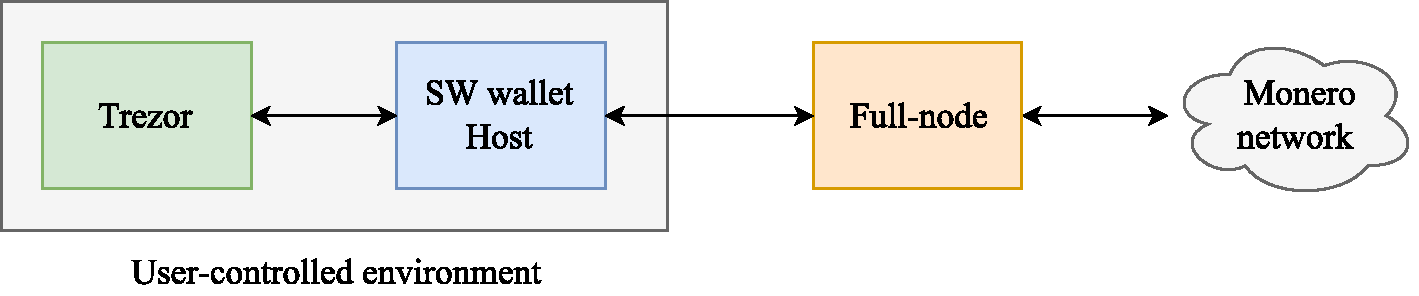
\includegraphics[width=0.6\textwidth, angle=0]{img/trezord.pdf}
	\caption{Environment}
\end{figure}


\subsection{License}
This work is part of the Monero to Trezor integration effort. This work is licensed under Apache v2 license in the current version. The license may change in the following revisions.

GitHub: \url{https://github.com/ph4r05/monero-trezor-doc} 

\subsection{Attacker model}

Trezor device attacker model is the same as with other crypto currencies (e.g., physical device security, memory forensics protection, side channel analysis, fault induction).

The host and the full node are assumed to be fully compromised. An attacker can start multiple instances of protocols, interleave protocol runs, send, replay, delay or drop any messages to/from the Trezor. Attackers goal is to spend user-unconfirmed transaction to his advantage or to cause any damage to the user leading to loss of funds. As the software wallet is operated from the host there are naturally no privacy guarantees on the host. Compromised host sees all transactions and can naturally block some messages, e.g., incoming transactions. 

In a weaker setting, only the full node is assumed to be fully compromised. The goal of an attacker on the full node is either to spend a victims monero, cause a loss or to learn any information about user's received or sent transactions (e.g., transaction ownership, balance, outgoing transaction addresses).
 
\subsection{Definitions}

\paragraph{Basic system}

\begin{itemize}
	\item $G$ is a base point of the curve $E$ (ed25519) of the order $l$
	\item $H_p : \{0,1\}^* \rightarrow E$, hash function to a curve point\footnote{\url{https://github.com/monero-project/research-lab/blob/master/whitepaper/ge_fromfe_writeup/ge_fromfe.pdf}}. 	
	\item $H_s : \{0,1\}^* \rightarrow [1, l-1]$, hash function to a scalar
	\item $H = H_p(G)$, a point on the curve $E$. It holds $H=hG$, where $h$ is unknown
	\item Points on the curve are denoted with capital letters, scalar values with lower case letters.
	
\end{itemize}

\paragraph{Transactions}

\begin{itemize}
	\item $(a, B)$ account view-key
	\item $(a, b)$ account spend-key (private scalars)
	\item $(A, B)$ the public wallet address, $A=aG$, $B=bG$
	\item $(C_{i,j}, D_{i,j})$ public sub-address with $i, j$ major minor index resp.
	\begin{enumerate}
		\item $D_{i,j} = B + H_s('SubAddr' \; || \; a \; || \; i \; || \; j)G$
		\item $C_{i,j} = aD_{i,j}$ 
	\end{enumerate}
	\item A single transactions has zero\footnote{Coinbase transaction has zero inputs, represents coin emission from the mining.} or more inputs; one or more outputs.
	\item $(r, R)$ transaction key-pair. Randomly generated per transaction. 
	\item $(x, P)$ transaction output spend key and an address. Unique per transaction output.
	\begin{enumerate}
		\item $x = H_s(rA) + b$, also called the ephemeral key. Used for spending.
		\item $P = xG = H_s(rA)G + B$, public key stored in the transaction output.
	\end{enumerate}
	\item $aR$ is also called the derivation (ECDH)
	\item \emph{mixin} is a number of additional decoy transaction outputs added to the unspent transaction output in the Ring signature.
\end{itemize}

EC points and scalars occupy 32 B.

There are field names from the JSON transaction representation used in the notation throughout the text.\footnote{Example: \url{https://xmrchain.net/tx/599533a7e42e82aa23c8da1d730fec047915ee5614556883cdce90739f1a94d3/1}}. There are also used variable names used in the Monero code base.

\paragraph{Abbreviations}
\begin{itemize}
	\item Transaction is shortened to \emph{TX} or \emph{TSX}.
	\item \emph{UTXO} stands for unspent transaction output, i.e., received monero usable for spending.
\end{itemize}

\subsection{Environment}

The basic setup is a Trezor hardware wallet with the account keys and a connected host.
We start with the most straightforward setup:
\begin{itemize}
	\item The host is running a Monero software wallet \verb|monero-wallet-cli|
	
	\item  The software wallet is connected to a Monero full-node (local or trusted remote).
	
	\item The basic wallet operations are performed via \verb|monero-wallet-cli| which is configured to work with the Trezor device.
	
	\item Some of the operations are performed inside the Trezor. 
\end{itemize}

Later, also the monero-gui wallet will be extended to support the Trezor.

\subsection{Account secrets.}
Account key-pairs are BIP-44 generated from the seed. Spend-key never leaves the Trezor device. There are two variants w.r.t. the view-key $a$:

\begin{enumerate}
	\item Performance BC scanning: view-key is exported to the host-based watch-only wallet to do the blockchain transaction scanning on behalf of the Trezor device. Watch-only device stores list of UTXO (unspent transaction outputs), i.e., received monero.
	\item Private BC scanning: view-key never leaves the Trezor device. The blockchain scanning is performed inside Trezor. 
\end{enumerate}

All other wallet related data, e.g., outputs with received moneros are
stored in the wallet on the host.

\subsection{Initialization} 
The wallet can be either created from a fresh seed or recovered from an existing seed.

The fresh wallet can be used right-away while the recovered wallet has to rescan the blockchain to detect all incoming transactions since the original wallet create-time (if unknown, the whole blockchain).

\section{Blockchain scanning}

In order to receive incoming transfers, the blockchain has to be scanned. A~specific operation has to be performed on each transaction output with the view-key $a$ to determine whether the transaction output is destined to us.

For a received transaction output Tx we have public keys $\left(R, P\right)$.
The wallet computes: 

\begin{equation}
B^\prime = P - H_s(aR)G
\end{equation}


If $\left(B^\prime = B\right) \; \vee \; \left(B^\prime \in \{D_{i,j}\}_{i,j}\right)$, then\footnote{$B^\prime$ is equal to the user's $B$ or one of it's sub-addresses} the transaction output is destined for us. Otherwise it can be ignored by the wallet.

Computation complexity per each transaction output: 2x point multiplications, 1x SHA-3, 1x point subtraction.

\subsection{Sub-addresses}
The sub-address is defined by the base address $(A,B)$ and the index tuple $(i,j)$, unsigned 32 bit major and minor index \cite{mrl_006_subaddr}.

\begin{itemize}
	\item The $(C_{i,j}, D_{i,j})$ is sub-address with major index $i$ and the minor index $j$.
	
	\item  The wallet holds mappings $D_{i,j} \rightarrow (i, j)$ and $(i, j) \rightarrow D_{i,j}$. 
	
	\item According to the convention, the master address has indices $(0, 0)$.
	
	\item Public key for sending transaction to sub-address: $P = H_s(rC_{i,j})G + D_{i,j}$
	
	\item Private spending key: $x = H_s(aR \; || \; idx) + b + H_s('SubAddr' \; || \; a \; || \; i \; || \; j)$, where $idx$ is a real transaction output index in the transaction as transaction can have multiple outputs.
	
	\item The blockchain scanning works with the same formula, no extra computation is needed. The wallet only needs to pre-compute all public spend keys which is done in advance. The protocol is backward compatible with standard addresses. For the proof check she Sub-address protocol proposal \cite{mrl_006_subaddr} for details.
\end{itemize}

\subsection{Performance scanning} 
The view-key $a$ is exported to the software wallet. For the receiving, no Trezor interaction is needed. 

\noindent Pros:
\begin{itemize}
	\item High-speed synchronization.
	\item Receiving moneros and balance without a need to have Trezor connected.
	\item Only small code changes required in the official Monero wallet.
\end{itemize}

\noindent Cons:
\begin{itemize}
	\item Permanent privacy loss. Host malware can read all future incoming inputs and the amounts. All wallets have to be assumed being public due to possible view-key leakage by the compromised host - even one time compromitation is enough.
	\item View-key exfiltration. The transactions can be revealed long after the compromitation is cleared. E.g., in court, blackmailing rich wallets, ...
	\item Inability to create short-lived wallets with the view key destruction after the wallet looses its purpose. 
\end{itemize}

\subsection{Private scanning}
The view-key $a$ never leaves the device. The device has to be connected
to perform the wallet refresh. 
Each new transaction has to be sent to the device for the identification.
There are several possible variants with varying complexity and performance.

\subsubsection{Naive approach} One roundtrip per transaction output to determine the ownership. 
\begin{enumerate}
	\item Send $(R, P)$ to the Trezor
	\item Trezor returns $B^\prime$, where $B^\prime = P - H_s(aR)G$
\end{enumerate}

If the host finds a match with $B^\prime$ it performs additional roundtrip to determine the transaction output value for RingCT transactions.

This is the most straightforward approach also suggested in the Ledger proposal \cite{ledger_doc}. The performance can be significantly degraded due to high computation and communication overhead. Although a benchmark would be needed to determine the baseline performance.

In terms of implementation this is a rather simple way as only the low-level operations are proxied to the HW wallet leaving most of the original code intact.

Communication complexity: One round-trip per transaction output. A transaction can have multiple outputs, block contains more transactions so multiple round-trips per one block refresh. The request is 64~B in size, response 32~B.

\subsubsection{Fast batched scanning}
During the wallet refresh the wallet loads missing blocks from the full-node RPC server. Each query yields 1000 blocks at maximum. 

The host wallet sends a batch of transaction outputs to decide the ownership in the Trezor. This part is called a \emph{transaction output identification}.

\begin{enumerate}
	\item Choose a batch size $bt$
	\item Create a list $lst = [(R_k, P_k), (R_{k+1}, P_{k+1}), ...]$ such that $|lst| \leq bt$
	\item Send $lst$ to the Trezor
	\item Initially, Trezor sets $res = []$
	\item Trezor processes each $(R_i, P_i)$. If there is a match, the index is added to the result array $i \rightarrow res$.
	\item Trezor returns $res$ 
\end{enumerate}
Most of the time the Trezor will just return an empty list as there is no new incoming transaction output destined to the account. If the list is not empty then the detailed scanning is performed for each transaction. 

Communication complexity: One message roundtrip per the batch. The request is $64bt$~B in size. The response is maximally $2bt$~B in size while the expected value is close to zero with overwhelming probability. 

\paragraph{Detailed scanning:} In this phase the host wallet sends transaction previously identified as belonging to our account for processing to the Trezor. The whole transaction output is sent to the Trezor so it can extract the amount and the mask from the transaction.

\paragraph{Sub-addresses:}
A wallet can generate independent-looking sub-addresses that are usable for receiving moneros using the same secret keys. Over the time wallet generates and stores multiple sub-addresses. 
For a recovered wallet sub-addresses are pre-computed in advance, $10k$ in total (look-ahead limits $L_M, L_m$, where $L_M=50$ and $L_m=200$ in the current version).
This poses a problem for the private BC scanning on the Trezor if the number of sub-addresses is large as the Trezor needs to decide transaction ownership using the sub-addresses set\footnote{The set of size several thousands of address may be difficult to store in the device}.

There are several workaround variants for the transaction output identification. The request remains the same as in the previous protocol. The batch of $(R_i, P_i)$ per transaction output.

\begin{enumerate}
	\item The Trezor returns a list of results $\left[B^{\prime}_k, B^{\prime}_{k+1}, \dots\right]$ instead of the index list. The decision is then made on the host. Each point has 32 B in size. This variant increases a communication overhead as each transaction output yields $B^{\prime}_i$.
	
	\item The Trezor returns a list similarly as in the previous variant with a difference of sending prefix of the fixed size $p_s$
	$\left[\text{prefix}_{p_s}\left(B^{\prime}_k\right), \text{prefix}_{p_s}\left(B^{\prime}_{k+1}\right), \dots\right]$. Host matches the prefixes with the internal prefix database. If a match is found, transaction is sent for detailed scanning (as before). Trezor might return null as a false positive hit.
	
	\item Trezor builds an internal mapping: $\text{prefix}_{p_s}\left(D_{i,j}\right) \rightarrow \left[(i, j), \dots\right]$.
	If the Trezor finds a prefix match it computes the full sub-address for all matched indices $(i,j)$ to decide false-positive vs. match. Then it returns a list $\left[(idx_1, (i_1, j_1), (idx_2, (i_2, j_2), \dots)\right]$ with all matched results to the host. 
	
	\item Use Bloom filter\footnote{ \url{http://llimllib.github.io/bloomfilter-tutorial/}, \url{https://en.wikipedia.org/wiki/Bloom_filter}} to optimize the storage of the sub-addresses. Bloom filter is a probabilistic data structure for checking the set membership returning results: maybe, no.
	This method enables to balance false positive hits with memory storage. For number of sub-addresses $n=10000$, bit-size of the Bloom filter $m=100000$ the optimal number of hash functions $k=\frac{m}{n}ln2 \approx 7$, false positive probability is roughly $\left(1-e^{-kn/m}\right)^k \approx 0.0084$, $8$ false positives in $1000$ tests with memory requirements $12.5$~kB.
	
\end{enumerate}

\subsubsection{Summary}
Ledger Monero Wallet is using the private blockchain scanning one transaction at a time \cite{ledger_doc}. Without further optimizations, this can be rather slow for the wallet refresh in terms of computations and bandwidth.
We conclude that our improvements (batching) are viable alternatives for privacy-sensitive users.

\noindent Pros:
\begin{itemize}
	\item The view-key $a$ never leaves the device.
	\item $a$ cannot be exfiltrated from the compromised host. Transaction attribution is leaked only during active compromitation.
	\item The same security-level as the Ledger.
\end{itemize}

\noindent Cons:
\begin{itemize}
	\item Slower wallet synchronization.
	\item Wallet restore could be infeasible as the whole blockchain has to be scanned (or take hours or days to complete). Benchmark is needed for this.
	\item More code changes required in the existing software wallets to implement the batching. The naive approach can be implemented with minimal changes (proxying $aR$ operation to the device).
	\item Inputs and the amounts still visible on the host.
\end{itemize}

\subsubsection{Extension} In order to further increase the privacy we could hide all transaction inputs on the hosts, to protect the balance value. The balance would be visible only on the Trezor device on request.

The extension would complicate the transaction creation a bit. The Trezor would have to work with the (possibly all) inputs when creating a new transaction. The whole transaction would have to be built in the Trezor. This is rather complicated in terms of implementation. Possible challenges: outputs storage (available flash memory on Trezor vs. encryption when stored on the host), secure memory access - protect from access pattern leakage.

\subsection{Updates}

\paragraph{12\textsuperscript{th} Feb 2017:} Performance version is chosen for the blockchain scanning. Privacy version can be implemented later.

\section{Sending a transaction}
Assume we are going to send $xmr$ Moneros to the address $(A_d, B_d)$
Overall, the sending process goes like this (description inspired by Ledger proposal \cite{ledger_doc}):

\begin{enumerate}
	\item Generate a transaction key-pair $(r, R)$
	\item Process a stealth payment ID
	\item Randomly select received non-spend transaction outputs to spend $T_{in}$ covering the $xmr$ + fee.
	\item Find $mixin$ fake outputs\footnote{get\_outs()} for each UTXO\footnote{unspend transaction output} $T_{in}$ to get ring size $mixin + 1$.
	\item Load the transaction information $(P_i, C_i)$, public key (address) and the amount commitment, from the full-node RPC server for the real and fake outputs going to spend.
	\item For each input transaction $T_{in}$ and each UTXO to spend $T_{in,i}$:
	\begin{enumerate}
		\item Compute a derivation $\mathcal{D}_{in,i} = aR_{in}$
		\item Compute an ephemeral tsx spend key $(x_{in,i}, P_{in,i})$, \\where $x_{in,i} = H_s(\mathcal{D}_{in,i} \; || \; \text{varint}(i)) + b$, where $i$ is the index of the UTXO in the transaction $T_{in}$
		\item Compute a key image $I_{in,i} = x_{in,i}H_p(P_{in,i})$
	\end{enumerate}
	\item Build the set of output transactions $T_{out}$. Typically there is one transaction to the $(A_d, B_d)$ address.
	\item If input $>$ output + fee, create a change transaction $T_{chx} \rightarrow T_{out}$. 
	\item For each transaction output $T_{out}$:
	\begin{enumerate}
		\item Compute the range proof. Borromean or Bulletproof \cite{monero_1098, borromean, Bnz2017BulletproofsSP}.
		\item Mask the output amount and the commitment mask in the \verb|ecdhInfo|\footnote{\url{https://github.com/monero-project/monero/blob/a9421f78027dbbdfe82420a5c6f7e77eb4c80bf4/src/ringct/rctSigs.cpp\#L688}} with the secret $H_s(aR\; || \; idx)$ denoted as the amount key.
		\item Compute the output commitments: $C = a_mG + xmrH$, where $a_m$ is a randomly generated commitment mask.
	\end{enumerate}
	\item Compute RingCT MG for each $T_{in}$ (real + fake inputs).
	\item Submit the transaction.
\end{enumerate}

\paragraph{Observations:}
\begin{enumerate}
    \item The transaction key pair $(r,R)$ should be generated in the Trezor to make sure it is random and not re-used (attacks by crafting $r$ on the host to leak the information). 
	
	\item The $T_{in}$ processing requires private keys - has to be done in Trezor. Trezor could display sum of all inputs. The transaction can be spent with the $x_{in}$, thus it must not be leaked to the host.
	
	\item The change address has to be generated in the Trezor to avoid the change address spoofing by the compromised host (sending a huge change to the attacker in the transaction confirmed by the user).
	
	\item Each transaction output $T_{out}$ and the monero amount has to be manually confirmed on the Trezor to finish the transaction processing.
	
	\item The range proof does not work with any secrets so it can be offloaded to the host. Range proofs are quite expensive operations and take up to 80\% of the whole transaction space\footnote{Bulletproof takes less space}. Implementation in the software wallet is significantly simpler and faster.
	
	\item Output commitments do not require secret keys but the computation is rather simple so can be performed in the Trezor.
	
	\item The final Ring signatures on inputs will be performed in the Trezor.
\end{enumerate}

\paragraph{Ledger comparison.} The Ledger proposal \cite{ledger_doc} goes further with the protocol modification by employing a custom sub-division protocol. Due to a hardware nature of the Ledger Nano S (which uses ST31H320 secure element, with 10~kB user RAM \cite{hw_wallet_vulns, st31h320}) it is not feasible to compute the transaction in the Ledger in one step so a multi-step approach had to be chosen.

The majority of transaction building process is performed in the software wallet while only the low-level crypto operations with the secret keys are performed in the Ledger.  

The sensitive sub-results are returned sealed to the software wallet, encrypted by simple AES/ECB encryption with transaction-specific encryption key, so the sensitive values cannot be used beyond the transaction scope. Ledger has to unseal the inputs, perform the operation and reseal the outputs before returning the result to the wallet. Moreover, to protect the protocol integrity the inputs are hashed in the Ledger. 

\;
\noindent Pros:
\begin{itemize}
	\item Rather simple implementation. The software wallet performs the heavy-lifting while some of the 
	low-level crypto calls are proxied to the Ledger. The sealing is format preserving so no data structures augmentation is needed. Code modifications are small.
	\item Device holds the minimal transaction state.
	\item Abstract device interface in the official Monero code. The plan is to support more HW devices.
	\item The protocol is already designed. We could alleviate an existing PR\cite{ledger_pr} in the Monero wallet.
\end{itemize}

\noindent Cons:
\begin{itemize}
	\item Protocol design is still evolving. Has not been merged yet.
	\item Sound security analysis of the protocol subdivision is missing. 
	\item The partial protocol can be vulnerable e.g., to change address attacks.
\end{itemize}

\subsection{Signing protocol}

The naive and the most straightforward variant is to adapt the Ledger design. On the other hand, the design is rather new and could be subject to further changes with high probability in the near future. 

Trezor has more resources available for the same job so I suggest doing as maximum as possible on the Trezor to avoid potential vulnerabilities from the protocol subdivision on the low-level.

\subsubsection{Transaction assembly algorithm}

The current version of the Monero software wallet may generate multiple pending transactions while only one is sent eventually in the process of assembling the inputs, outputs and the fee computation (e.g., \emph{wallet2.cpp:6940}\;\verb|goto skip_tx|). The fee is first estimated by a simple formula. However, the serialized transaction blob size precise estimation is problematic mainly due to \verb|VARINT_FIELD()|, variable length fields. So the transaction is fully assembled, signed and the real fee is computed as a function of transaction serialized blob. If the computed fee is higher than the  estimated value the transaction is recomputed, the old transaction is discarded. 

One could implement a precise fee computation algorithm but that would duplicate the serialization code which could lead to bugs when the structures are extended in the future. Thus it is easier and safer to build the transaction and then compute the blob size as we have only one code path working with transaction serialization. If serialization changes, the fee computation works without change. 

The software wallet does not have valid wallet keys and we don't want to involve Trezor in this assembly as it would pose unnecessary overhead. The fee computation will be done in the same way as it is now in the software wallet to avoid potentially inducing new bugs. Wallet creates a transaction in the same way but signs it with random account keys so the fee computation is precise.

Once the algorithm picks a correct transaction to send the user has to confirm all transaction outputs (including the change transaction). Once the transaction is confirmed the transaction is signed with real keys in the Trezor and returned to the wallet. After that, the transaction state is reset.


\subsubsection{High-level protocol description} 
All signatures are performed in the Trezor on the set of spending transaction outputs (TXO) in one step. Output range proofs are offloaded to the host as explained below.

Let $H$ be a cryptographic hash function $H : \{0,1\}^* \rightarrow \{0,1\}^{256}$, preferably Keccak-256 which is already used in the Monero. Let \emph{KDF} be the key derivation function which will be used to derive further HMAC and encrypton keys. The \emph{KDF} has 32 B output. In this paper it is assumed to be $H^2(x)$ which is equivalent to $H(H(x))$. HMAC uses the hash function $H$. Binary operator $||$ is a binary concatenation.

\paragraph{State:}
Trezor holds a transaction state:
\begin{itemize}
	\item Transaction data (inputs, outputs, $(r,R)$, range proofs, signatures, $\dots$)
	\item Transaction cryptographic material: master key $k_{mst}$, base HMAC key $k_{hmac}$
\end{itemize}

\paragraph{Protocol description:}

In the protocol description context $H$ represents a host and $T$ represents Trezor.
\begin{enumerate}
	\item $H \rightarrow T$: $TsxData = \text{payment\_id},\text{unlock\_time},  \left[\left(T_{out,i}, \text{amount}_i \right), \dots \right]$. Host sends the initial transaction data $TsxData$ to the Trezor by calling: \emph{InitTransaction}$\left(TsxData\right)$.
	
	\begin{enumerate}
		\item $T$: Reset the Trezor transaction state, store $TsxData$.
		
		\item $T$: Generate $(r, R)$, transaction key-pair.		
	\end{enumerate}
	
	\item $H \rightarrow T$: Set inputs to spend + loaded fakes $T_{in}$. 
	\begin{enumerate}
		\item $T$: For each input: compute derivation $\mathcal{D}_{in,i}$, ephemeral spending key $x_{in,i}$, key image $I_{in,i}$.
	\end{enumerate}
	
	\item $H \rightarrow T$: Set range proofs \emph{asig} for $T_{out}$. Optional, can be computed in the Trezor, may be slower. Useful for Trezor.io (web wallet implemented in JavaScript).
	\begin{enumerate}
		\item $T$: Store the range proofs.
	\end{enumerate}
	
	\item $H \rightarrow T$: Request the signed transaction $T$
	\begin{enumerate}
		\item $T$: Transaction sanity check
		
        \item $T$: Ask the user for confirmation.

		\item $T$: Compute output commitments
		
		\item $T$: Perform RingCT signatures on inputs $T_{in}$ (signs also the transaction prefix (inputs, outs, tsx pub key $R$, outputs range proofs, commitments)) with the $x_{in}$ and the key image $I_{in}$.
	\end{enumerate} 
	
	\item $T \rightarrow H$: Return the signed transaction $T$.
\end{enumerate}
%\improvement[inline]{Finish decription}


\subsection{Large transactions}
Simple transactions have roughly around 13.2 kB in size. With range proof offloading it is very easy to compute it completely in the Trezor. The problem can arise if a user wants to spend many small inputs to pay to multiple addresses and/or the mixin size is large, e.g., above 10. This increases memory requirements, once the threshold is reached it is not feasible to compute the transaction in the Trezor.

Note that the transaction outputs processing has to be finished in order to do a RingCT signature on the UTXOs as the signature contains hash of the outputs (range proofs), \emph{final\_message}. Each UTXO is RingCT-signed separately. The inputs to the signature are mainly:

\begin{itemize}
	\item \emph{final\_message} hash. Binds the transaction to the TXO signature (see below), has 32~B in size.
    \item Vector of $(P_i, C_i)$, the public keys and the commitments for the transaction inputs. One entry in the index is our UTXO to spend; others are decoys / mixins. The size is $(mixin+1) * 64$~B.
	\item Secret spending key $x_{in}$ and the mask $a_i$, together 64~B.
\end{itemize}
For data flow diagram see Figure \ref{fig:data_flow}.
The memory requirements for the signature input is $(mixin+1) * 64 + 96$~B in total.

The RingCT signature per one TXO contains a 32~B key field \emph{cc} and the matrix of 32~B keys called \emph{ss} having $2$ rows and $mixin + 1$ columns. The memory requirements for the output are then $(mixin + 1) * 64 + 32$~B.

\paragraph{Protocol subdivision}

Obviously, the one-step transaction construction may not suffice for large transactions with many inputs and large mixins. Thus in order to support arbitrarily large transactions, the subdivision has to be employed. The subdivision should undergo a security review before being deployed to the production. In the subdivided approach we do not stick to the Ledger proposal as we can go few levels up compared to the relatively low-level approach of the Ledger subdivision. E.g., compute the whole RingCT for one input in the Trezor. The minimal division unit is one input/output. 

Subdivision protocol works in an incremental manner. The transaction is being built on the host from information provided by the Trezor. Each input and output is processed one by one. In the last stage of the protocol the signature per input is generated. Once the protocol is finished the host has the complete transaction.

\paragraph{Memory consumption example:}
If the transaction has 30 TXOs with mixin set to 19 the overall memory requirements for inputs are 41~280~B, outputs are 39~360~B. This is the minimal memory needed to do the computation. The signature itself consumes roughly around 128~B of memory per TXO.

\subsection{RingCT MLSAG Signature details}

RingCT signature over the input from $T_{in}$ signs the input values and the message hash \emph{final\_message} binding all transaction data to the input being signed. A part of the \emph{final\_message} is the \emph{transaction\_prefix}:

\begin{lstlisting}[language=c++]
class transaction_prefix {
public:
  size_t   version;
  uint64_t unlock_time;  
  std::vector<txin_v> vin;
  std::vector<tx_out> vout;
  std::vector<uint8_t> extra;
}
\end{lstlisting}

Fields \emph{version}, \emph{unlock\_time} are simple primitive types defining the transaction version and the block-time the transaction can be spent. Fields \emph{vin}, \emph{vout} define all TXO to spend and destinations respectivelly. Field \emph{extra} contains transaction public keys\footnote{More than 1 if sub-addresses are used} and another serialized metadata, such as encrypted payment ID and additional transaction public keys if applicable (sub-addresses).

The transaction outputs \emph{tx\_out} is a tuple \emph{(amount, pub\_key)} for an ordinary outgoing transactions, sent by an user. 

The \emph{txin\_v} is a variant type\footnote{Similar to union, can have one of given types} but WLOG let's assume its type is \emph{txin\_to\_key} which is used with ordinary transactions. 

\begin{lstlisting}[language=c++]
struct txin_to_key {
  uint64_t amount;
  std::vector<uint64_t> key_offsets;
  crypto::key_image k_image;
}
\end{lstlisting}

The \emph{amount} is the real amount of the TXO to spend, even for RingCT transactions. RingCT amounts are zeroed out before the signature is performed to hide the values in the transaction header as it gets to the blockchain. Zeoring is also necessary so third parties can verify the signature as they don't know the amount values for RingCTs.
The vector \emph{key\_offsets} codes the TXO indices in the blockchain. They form a mix set. One of the TXO is our which we can spend; others are decoys.
The \emph{k\_image} is the key image for the mix ring. It depends only on the TXO being spent. Decoy TXOs do not affect key image value, obviously.

\paragraph{Final message hash} The final message hash has the following structure:
	
\begin{equation}  \label{eq:final_message_hash}
\text{final\_message\_hash} = H(H(\text{transaction\_prefix}) \; || \; H(\text{rctSigBase}) \; || \; H(\text{rangeSigs}))
\end{equation}

Final message is hashed from 3 independent components. This fact is used in the subdivided signing protocol for incremental hashing of the \emph{final\_message}. E.g., range proof is hashed to the third component even though \emph{rctSigBase} and \emph{transaction\_prefix} hashing is not finished which saves few protocol round trips.
The \emph{final\_message} hash is generated by \verb|get_pre_mlsag_hash()| in the official Monero code base.
For the exact structures definition please refer to the appendix \ref{sec:structs}.

\paragraph{Security implications}
The fact that RingCT signature signs \emph{final\_message\_hash} which includes the \emph{transaction\_prefix\_hash} gives quite strong security guarantees. In fact, the signed TXO can be spent only in the context of the given transaction. The signature cannot be re-used for spending in a different transaction as the verification would fail. This protects from the attack where an attacker takes a valid transaction, reassembles it and submits own tampered version instead of the valid one.

Thus if we can build the transaction prefix and its hash securely in the Trezor we can use the protocol subdivision on the transaction inputs, RingCT signing one input TXO at a time with the offloading result to the host. 

\paragraph{Memory requirements}
The \emph{version} and \emph{unlock\_time} take 16 B. The \emph{extra} fields can vary in size, in majority of cases it contains the serialized transaction public key 32~B, the 8~B payment ID. It may contain multiple public keys if sub-addresses are involved. If there is at least one sub-address (and not the only one) in the output transaction, there is an additional public key for each transaction output, 32~B per transaction. Which gives minimally $16 + 32 = 48$~B. In general it may be $56 + \left|T_{out}\right| * 32$~B.

The \emph{vin} takes roughly $(8 + 8 * (mixin + 1) + 32) * \left|T_{in}\right|$~B, ignoring the serialization overhead (tagging, array size encoding). The \emph{vout} takes roughly $(8 + 32) * \left|T_{out}\right|$.

The basic transaction with two inputs and two outputs and mixin 4 takes approximately $56 + (40 + 5*8)*2 + 40*2 = 296$~B. A more advanced case with 100 inputs, 100 outputs, and mixin level 99 yields 88~006~B.  

\subsection{Subdividing output processing}
We asume user inputs are scatered among many small input unspent UTXO while there are only small amount of transaction outputs. Thus inputs have to scale in size while outputs related data is stored in the transaction state.

Transaction prefix and its hash is computed in the Trezor.
For an easier description I use the field names used in the JSON transaction representation.\footnote{Example: \url{https://xmrchain.net/tx/599533a7e42e82aa23c8da1d730fec047915ee5614556883cdce90739f1a94d3/1}}

\paragraph{Intro to hashing}
All \emph{final\_message\_hash} components are hashed independently to reduce round trips and save the state memory on the device.
The \emph{tx\_prefix\_hash} is hashed during input and output processing. All inputs and outputs have to be processed in order to compute this hash.

The \emph{rctSigBase} has the following structure with respect to the hashing:  
\begin{lstlisting}[language=c++]
struct rctSigBase {
  uint8_t type;
  xmr_amount txnFee;
  std::vector<key> pseudoOuts;      // input amount commitment
  std::vector<ecdhTuple> ecdhInfo;  // outputs enc (value, mask)
  std::vector<ctkey> outPk;         // outputs (dst_key, commitment)
}
\end{lstlisting}

Unfortunately the structure \emph{rctSigBase} cannot be hashed incrementally in one pass (i.e., as inputs and outputs are processed) as it hashes whole vectors. Namely all \emph{ecdhInfo} have to be hashed from all outputs, then all \emph{outPk}. Fortunately, the ordering of the message fields is appropriate as it minimizes the memory needed to compute the hashing. The \emph{type} and \emph{fee} fields are initialized in when protocol starts. \emph{pseudoOuts} are hashed incrementally as inputs are processed. \emph{ecdhInfo} are hashed incrementally as outputs are processed and \emph{outPk} is stored to the transaction state. It is hashed after all outputs are processed. The field ordering is beneficial because \emph{ecdhInfo} is not needed after hashing anymore while \emph{outPk} is used in the signing.

The \emph{rangeSigs} structure can be hashed incrementally, one transaction output at a time so the range proof is hashed during creation.

\begin{figure}[H]
	\centering
	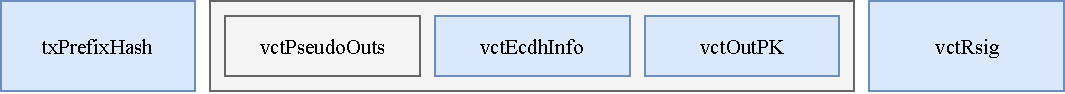
\includegraphics[width=0.8\textwidth,clip, angle=0]{img/premlsag_hash.pdf}
	\caption{PreMlsagHash computation.}
\end{figure}


VctPseudoOuts is hashed only for RctSimple transaction type. There are two different UTXO signature schemes, \emph{full} and \emph{simple}. The Full scheme is only used with single UTXO and only with Borromean range signatures. Otherwise the simple mode is used. The VctPseudoOuts is hashed only in the simple mode with the Borromean range signature. The simple mode with Bulletproofs has stored pseudo outputs in the prunnable part of the signature thus it is not hashed. 

For detailed structure definitions please refer to the Appendix \ref{sec:structs}. 

\subsection{Data offloading}
As HW wallets are resource constrained devices and cannot hold all required information in the memory for large transactions there is a need to offload data to the host during the transaction construction process. The offloaded data is then later passed back to the Trezor in the protocol.

Offloaded information can be either private or public. The public information is the one not leaking account secrets in the attacker model, i.e., information already known to the attacker, derivable from existing information or publicly stored in the blockchain. The example is key image, destination output address, etc... The private information is typically a commitment scalar mask.

Both types of offloaded information have to have an integrity protection (e.g., with HMAC) so the protocol gets the exact information it expects, preventing the attacker tamper the data, replay existing, etc...
The private offloaded data have to be also encrypted so the protocol does not leak sensitive information to the attacker or information not publicly known from the blockchain. Such leak could lead e.g., to a reduced security level or e.g., constructing proofs about the transaction to third parties which would not have been possible without the leak (privacy risk). The AEAD (authenticated) encryption is used to provide both confidentiality and integrity.


\paragraph{Public data offloading - HMAC}
To protect the transaction components integrity and ordering of the offloaded fields they are HMACed with the unique-purpose key so information from different protocol step cannot be reused. Key is constructed as follows:
\begin{equation}
\begin{split} \label{eq:det_mask}
k_{mst} &= \textit{KDF}(TsxData \; || \; r \; || \; \text{rand\_nonce})\\
k_{hmac} &= \textit{KDF}\left(\text{"hmac"} \; || \; k_{mst}\right)\\
k &= \textit{KDF}(k_{hmac} \; || \; \text{"txoutres"} \; || \; i)
\end{split}
\end{equation}

 Where $i$ is the index of the outgoing transaction output. By the construction each offloaded information has an unique HMAC key.

Once the HMACed data is loaded from the host the HMAC is checked. Thus attacker cannot tamper the data, reorder, reply or drop any output transaction data. During the HMAC verification, the index is computed by the Trezor, so the ordering of the transactions has to be preserved otherwise the HMAC will fail (no replay, reordering or skipping). No other transaction can be added as the HMAC will be invalid. Trezor has to check if none transaction was dropped.

\paragraph{Private data offloading - encryption}
On top of the integrity protection private data have to be encrypted.
The protocol uses Chacha20Poly1305 with unique purpose key as described earlier. Each offloaded item has a different unique encryption key.
The initialization vector (IV) is randomly generated by the Trezor. Key is derived as in the previous key, but with a different base key $k_{enc} = \textit{KDF}\left(\text{"enc"} \; || \; k_{mst}\right)$.

Note that from the key construction the IV could be also zero. As GCM mode does not have a padding this could be used to transparently encrypt offloaded fields without changing structure sizes. Zero IV variant is not used in the protocol.

As offloaded data are of the same size, the key is unique per offloaded entry and the Chacha20Poly1305 is secure the private offloading does not leak information. The authentication tag is checked before the decrypted value is used. If tag is not valid exception is thrown which leaves to erasing the transaction state.

\paragraph{Private data reconstruction} \label{mask_reconstruction}
Most of the offloaded private data is randomly generated scalar mask values, e.g., for the commitments. An alternative to offloading masks to the host is to generate them in a deterministic way and re-generate again when needed in the protocol. With this approach no offloading is needed which can save protocol round trips. The mask could be generated as in the equation \ref{eq:det_mask}. 
\begin{equation}
\begin{split} \label{eq:det_mask}
k_{msk} &= \textit{KDF}\left(\text{"mask"} \; || \; k_{mst}\right)\\
k_{msk,idx} &= \textit{KDF}\left(k_{msk} \; || \; \text{"rsig-rnd-ai"} \; || \; idx \right)\\
a[i] &= KDF(k_{msk,idx} \; || \; i \;) \; \text{mod} \; l  \\
\end{split}
\end{equation}

The key $k_{msk,idx}$ is created separately so it can be passed to the host for deterministic mask generation (if needed) without compromising the mask key $k_{msk}$.
The mask pre-image has to be unique so the value does not repeat and is not predictable. This scheme works in the random oracle model. The similar approach is used in Fiat-Shamir heuristic, in zero knowledge proofs. The output of a $H(\cdot)$ / Keccak-256 is assumed to be indistinguishable from a truly random number stream. The building block $H$ can be simply replaced by a stream cipher or block cipher in CTR which is also commonly used as the PRNG. Mask are 32 B values which needs to be reduced modulo curve order.

Usually, the masks are consumed sequentially during processing so another optimization is possible. To speed-up the mask generation a fast stream cipher can be used, i.e., it's \emph{keystream} output. By using e.g., \emph{Chacha20} one can get better performance for sequentially consumed masks by using key stream directly. The modular reduction is another intensive part but it is performed also for randomly generated masks so it is not optimized in the recomputation.

This approach can be implemented easily using polymorphism on item access. Vector object defines \\ \verb|__getitem__(self, item)| method which dynamically computes mask from the internal state. For the sequentially accessed masks it can reset the keystream if the index is zero. In this way the object behaves like normally generated mask so there are no changes to the other parts needed. 


\subsection{Range proof offloading}
Range proof could be potentially offloaded to the host to reduce computation time and the RAM consumption.
The offloading is mainly motivated by the fact it makes up the significant portion of the transaction (per output) in size. The simplest Monero transactions with only two input and two outputs (change address) have around 
13.2~kB where the range proof constitutes about 12~kB from the total size for Borromean range proof. \footnote{\url{https://getmonero.org/2017/12/07/Monero-Compatible-Bulletproofs.html}}

Range proofs are computationally expensive and not using any account or transaction secrets. Offloading thus poses no additional security risk in the current attacker model. However, if the attacker generates masks in a predictable way it could lead to leaking amount being sent from the range proof stored on blockchain. This poses potential privacy risk as the attacker could potentially prove the amount to a third party from the blockchain (e.g., for court). The attacker on its own already knows the amount as the output addresses and amounts are entered on the attacker-controlled host.

The offloading idea is demonstrated mainly on the Borromean range proofs as they are of significant size, but it also generalizes to the Bulletproof (the same interface). 
The range proof is a zero-knowledge proof that the amount lies in the interval $[0, 2^{64})$ without revealing the amount value\footnote{To protect from a negative overflow which would generate new Monero - required part of confidential transaction mechanism using Pedersen commitments.}. Intuitively, the invalid range proof causes only the transaction rejection by the full node without compromising the security.

Range proof is generated by \verb|proveRange()| in \emph{rctSigs.cpp:298}. The only input value to the function is \verb|const xmr_amount & amount|, the amount. The function returns \verb|rangeSig| structure with the range proof, the mask and the amount commitment. 

\paragraph{Offloading separation.}
The first part of the \verb|proveRange()| function generates random $a_i$ scalar mask values and computes $C_i$ commitments which are further used to generate range proof signatures. These values are generated in Trezor to ensure the proper randomness as $a_i$ are used as amount commitment masks. Mask values are protected from tampering in this design. Masks occupy $32*64~B = 2~kB$ RAM. 
The deterministically masks approach described in \ref{par:det_masks} may be used to minimize transfer data.

%\paragraph{63-of-64}. With the maskign used attacker knows also the overal amount masking value from Pedersen commitments for transaction outputs. 

\paragraph{Sending a transaction.}
Assume the attacker generates an invalid range proof or a range proof for an invalid amount value. The range proof is included in the overall message hash, the \emph{final\_message}, which is signed by the RingCT signatures. Besides that, the range proof values \emph{asig} are not used in the transaction construction. Thus an invalid range proof does not affect the value commitments. 

The full-node validates the whole transaction once the transaction is received to the pool. It is not possible the transaction with invalid range proof is added to the blockchain. The node signalizes an error and transaction is rejected.

In the attacker model, the host already knows the amount as a legitimate user uses software wallet to enter the amount when sending the transaction the privacy is not lost.

\paragraph{Receiving a transaction.}
In the attacker model, the host can already tamper the range signatures thus offloading does not make any difference.
WLOG assume we are using simple RCT\footnote{Non-simple RCT is a bit smaller in size while usable only if the transaction is of a certain form. This alternative does not affect the range proof.}. The range proof verification function is \verb|verRange()| which is called only in the \\\verb|verRctSimple()|. In the current version only full-nodes do RCT verification during the refresh, not the wallet. If the transaction verification fails, it is ignored.

\paragraph{Memory requirements.} 
The range proof consists of Borromean signature and an array of 32~B commitments $C_i$ with 64 elements, one for each bit in the amount value. The Borromean signature contains: $2$ arrays \emph{s0}, \emph{s1} each with $64$ keys, each 32~B, and one 32~B key. In total, the range proof with commitment takes 6176~B in the raw form per one transaction output.

\subsection{Bulletproof}\label{sec:bp} The offloading mechanism is very similar to the Borromean range proof. The random mask and the amount commitments \verb|V| are computed in the Trezor to make sure it was not tampered with (simple computation step with amount and mask). 
By switching to Bulletproof the range proof size for 2 outputs is reduced roughly from 12~352~B to 2~500~B as Bulletproof signs all outputs with a single signature. The offloading is not required with Bulletproof if each output transaction has own Bulletproof \cite{Bnz2017BulletproofsSP}. However, if batched bulletproof are used the memory requirements for the computations increase so it cannot be computed on the device anymore. 

\paragraph{Batched Bulletproof} 
In the new Monero fork the batched Bulletproofs are implemented. Batched Bulletproofs are ZK proofs about multiple statements in a single proof. The proof size increase is logarithmic in the number of statements and statement sizes. Statement is a range proof about the transaction output value. Batching can cover the whole transaction with one BP. Note the BP can prove $2^x$ statements so if transaction has 5 statements the BP proof is of equal size as for 8 statements.

Log example: BP for one transaction output, L, R fields have 6 scalars. BP for two transaction outputs has 7 scalars in L, R fields so space saved is significant. Verification times are also better for batched Bulletproofs.

Here follows Bulletproof transaction types:
\begin{itemize}
	\item {\it RangeProofPaddedBulletproof}: This aggregates all transaction outputs to a single BP for the whole transaction. It is a default choice in the \verb|wallet2| for BP type if transaction. BP can currently aggregate at most $16$ transaction outputs (constant, technically could go bigger but memory allocations would grow). Padded means the BP is padded with dummy statements to the next power of two.
	
	\item {\it RangeProofMultiOutputBulletproof}: BP batching $2^x$ outputs up to the upper bound $16$. Transaction can have multiple BP of this type so it can effectivelly prove certain amounts of statements. E.g. 9 are with 1 BP for 8 statements and 1 BP for 1 statements. In the previous case BP for 16 statements would have to be used.
	
	\item {\it RangeProofBulletproof}: One BP per transaction output. In the current version it is used only for transactions with one output which is technically the same as {\it RangeProofPaddedBulletproof}.
\end{itemize}

\paragraph{Offloading} As the batched version allocates several 32~B key vectors of size $M\cdot N  = numOutputs \cdot 64$ the computation in the constrained environment is problematic for transaction with 2 and more outputs so offloading is necessary. Note the output value mask commitment $a_i$ is denoted \verb|$gamma_i$|.

The BP has the following structure:
\begin{itemize}
	\item Points/scalars \verb|A, S, T1, T2, taux, mu, a, b, t|
	\item Vector of commitments \verb|V| of size $M$
	\item Vector of points \verb|L, R| of size $log(MN)$
\end{itemize}

\paragraph{Secure offloading} is perfomed in the following way:

\begin{itemize}
	\item All output masks $a_i$ are generated on the Trezor before any range proof is computed, sent to host. Commitments $C_i = a_iG + \text{amount}_i H$ are computed in Trezor.
	
	\item Host generates batched BP with defined masks, the $C_i$ is the same as computed in the Trezor.
	
	\item Host sends the whole BP to the Trezor for verification and hashing to the PreMlsagHash. Note the commitment vector \verb|BP.V| is not part of the transaction and rsig PreMlsagHash as it is recomputed from \verb|outPk.mask|. On receiving the BP the Trezor performs BP verification with recomputed $C_i$. If verification succeeds, the host had to use correct commitment. The hash of the BP is computed for the PreMlsagHash. The BP verification is quite fast with small memory requirements compared to BP generation.
\end{itemize}

In the offloading scenario the attacker knows the commitment mask $a_i$ which can be leaked and used to prove some knowledge about the blockchain transaction.

\paragraph{Hardened offloading}
The host attacker could still generate masks 
\verb|sL, sR| maliciously so the proof will be valid but could leak attacker specified information to the blockchain. To minimize the attack surface the offloading can be hardened.

The hardened variant uses deterministic scalar values, i.e., generated by exact specification by secure KDF so attacker cannot generate own malicious masks.

\begin{itemize}
	\item \verb|BP.A| can be easilly and effectively computed on the Trezor to verify the \verb|alpha| mask and \verb|V| commitment.
	
	\item \verb|BP.S| can be also computed on Trezor to verify mask vectors \verb|sL, sR| and \verb|rho| are generated according to the specification.
	
	\item There are only two more random scalars generated by the prover, \verb|tau1, tau2| which propagate to \verb|BP.T1, BP.T2| but the direct verification of those is out of reach as they are generated in the most RAM intensive part of BP generation so Trezor could generate the whole BP proof.
\end{itemize}

\paragraph{Mask hiding hardening}

As seen from the algorithm \ref{alg:bp_mask} it is not trivial to hide a commitment mask $\gamma$ from the host in the offloaded BP generation. Trezor could generate the commitment vector $V$ which hides the mask $\gamma$ but the mask is also used for $\tau_x$ computation. In order to protect $\gamma$ and ensure all masks are properly generated the Trezor have to evaluate the BP prefix algorithm in $O(max(log(N), M))$ so it is practically usable. In order to protect $\gamma$ the masks $\alpha, \rho$ have to be generated randomly so attacker cannot compute $\gamma$ from $\tau_x$.

\makeatletter
\xpatchcmd{\algorithmic}{\itemsep\z@}{\itemsep=0.5ex plus2pt}{}{}
\makeatother

\begin{algorithm}[]
	\caption{Pseudocode of the first BP part. $\gamma$ is used only in the formulas in the algorithm. Value $x$ is result of a complex computation from the amount and constant values. } \label{alg:bp_mask}
	\begin{algorithmic}[1]
		\Function{BulletproofPrefix}{$amounts, \gamma$}
		\State \Comment{BP: $(V, A, S, T1, T2, \tau_x, \mu, L, R, a, b, t)$}
		\State $Gi_j \gets \text{getExponent}(H, 2j + 1)$ \Comment{Precomputed const}	
		\State $Hi_j \gets \text{getExponent}(H, 2j)$ \Comment{Precomputed const}	
		\State $V_j \gets \gamma_j G + amounts_j H$
		
		\State \Comment{Compute A}
		\State $aL, aR \gets \text{expandAmount}(amounts)$
		\State $\alpha \gets \text{randScalar}()$
		\State $A \gets 8^{-1} \left( \alpha G + \sum_{i=0}^{MN-1} aL \cdot Gi_i + aR \cdot Hi_i\right) $
		
		\State \Comment{Compute S}
		\State $sL, sR \gets \text{deterministicMasks}()$	
		\State $\rho \gets \text{randScalar}()$
		\State $S \gets 8^{-1} \left( \rho G + \sum_{i=0}^{MN-1} sL \cdot Gi_i + sR \cdot Hi_i\right) $
		
		\State \Comment{Compute y, z, taux}
		\State $y \gets H(H_s(V), A, S)$
		\State $z \gets H_s(y)$		
		\State \Comment{Vectors $l_0, l_1, r_0, r_1$ have $MN$ elements}
		\State $l_0 \gets aL - z$
		\State $l_1 \gets sL$
		\State $zt[i] \gets z^{2 + \floor{i/N}} 2^{i \% N}$
		\State $r_0[i] \gets ((aR + z)[i] * y^{i}) + zt[i]$
		\State $r_1[i] \gets sR[i] * y^{i}$
		\State $t_1 \gets (l_0 \cdot r_1) + (l_1 \cdot r0)$ \Comment{$t_1, t_2$ Computed simultaneously in one pass}
		\State $t_2 \gets l_1 \cdot r_1$ 
		\State
		\State $\tau_1, \tau_2 \gets \text{randScalars}(2)$
		\State $T_1 = 8^{-1} \left(t_1H + \tau_1G\right)$
		\State $T_2 = 8^{-1} \left(t_2H + \tau_2G\right)$
		\State $x \gets H(z, z, T1, T2)$ 
		\State $\tau_x \gets \tau_1 x + \tau_2 x^2 + \sum_{i=0}^{M} \gamma_i z^{i+2}$
		\State $\mu \gets \rho x + \alpha$
		\State \Return $(V, A, S, T1, T2, \tau_x, \mu)$
		\EndFunction	
	\end{algorithmic}
\end{algorithm}

Computing $t_1, t_2$ as inner products of $l_0, l_1, r_0, r_1$ is implemented in one pass over $N$, each element of vectors is accessed exactly once. This enables effective streamlined operation as the $t_1, t_2$ can be computed completelly in memory, thus the BP prefix can be computed in $O(1)$ memory.

Offloading protocol computes the BP prefix $(V, A, S, T1, T2, \tau_x, \mu)$ and returns to the host: BP prefix, $x, y, z$. The host can recompute $l_0, l_1, r_0, r_1$ and finish the BP.

\paragraph{Implementation optimizations}
The current Python implementation uses several optimizations to reduce the memory usage and allow several CPU/RAM tradeoffs:
\begin{itemize}
	\item Some constants and vectors are precomputed and stored as a byte string which is frozen\footnote{\url{http://docs.micropython.org/en/v1.9.3/unix/reference/constrained.html}} in the flash memory, not occupying memory. The byte arrays are wrapped by a polymorhpic memory access vector \verb|KeyV| so the usage and API is the same as with the normally computed vectors.
	
	\item Some vectors are dynamically evaluated instead of the precomputation. E.g., \verb|aL, aR| vectors derived from the amount are evaluated on the fly as function accesses the particular element. This reduces memory usage from $O(MN)$ to $O(1)$. CPU overhead is minimal.
	
	\item Random mask vectors \verb|sL, sR| are recomputed on each access. The memory is reduced from $O(MN)$ to $O(1)$ but there is a CPU tradeoff as the derivation and modular reduction has to be performed on each access. However, the constant is small, $[2,4]$.
	
	\item More complex vectors are evaluated on the fly if the element computation requires only constant amount  of RAM (typically 1 element) and CPU overhead constants are acceptable. E.g., vectors in the form $r_i=a_i+b_i$. 
	
	\item Vectors with sequential element access (basically most of them) are evaluated on the fly if the CPU overhead is acceptable and the memory required is constant in the sequential access, e.g., if $x_i = op(x_{i-1}, \text{constData})$. On $x_0$ access the state is reset. This is useful for vector of powers of some constant element $c$.
	
	\item Some constant vectors are precomputed for some prefix, matching BP size of 2 or 4 statements. If the higher index is accessed it is computed on the fly. Vectors precomputed in this way are \verb|GI, HI, TWO_N|. In case of vector of powers of 2 the precomputed part is re-used to compute the result. One such vector is $maxM \cdot 64\cdot32$~B long and frozen in the flash.
	
	\item Slices of vectors are computed as constant views to existing wrapped vector, memory overhead $O(1)$.
	
	\item Optimizations can be chained if the operations does not have conflicting dependencies. So typically unary operations or x-arry operations with constants / non-conflicting dependencies.
	
\end{itemize}

It is also required to reduce memory allocations so the heap framentation is minimized. For this purpose all computations reuse statically allocated buffers / vectors.

By using these tricks it is possible to compute a bit larger BPs on the Trezor but the computation time would be rather high. The memory complexity is currently $(4MN \cdot 32) + O(max(lg(N), M))$, due to data dependencies. Verification algorithm is memory optimized and runs with $O(max(lg(N), M))$ memory.

The size of the proof itself is $32(9 + M + 2log(NM)) = 32(21 + M + 2log(M))$, for $N=64$ bits of amount and $M$ statements. 

\begin{table}[H]
	\caption{BP performance on the Trezor. Test were run with precomputed vectors for $4$ statements. Statements 8 and 16 were not computed due to low amount of RAM.}\label{tbl:bpperf}	
	\begin{center}
	\begin{tabular}{p{3.5cm} rrrrr}
		\hline
		Prover outputs       & 1         & 2       & 4      & 8      & 16      \\ \hline
		Time (s)             & 10.05     & 18.08   & 34.24  &      - &       - \\
		RAM min (B)          & 8 192     & 16 384  & 32 768 & 65 536 & 131 072 \\
		RAM (B)              & 12 704    & 21 056  & 38 112 &      - &       - \\
		\hline\hline
		
		Verifier outputs  & 1         & 2       & 4      & 8      & 16     \\ \hline
		Time (s)          & 3.18      & 6.07    & 12.00  & 25.36  & 52.45  \\
		RAM (B)           & 9 216     & 9 920   & 7 760  & 8 864  & 10 496 \\ \hline
		
		Proof size (B)       & 704       & 800     & 928    & 1120   & 1440    \\
		Borromean equiv. (B) & 6 176     & 12 352  & 24 704 & 49 408 & 98 816  \\ \hline
		
	\end{tabular}
	\end{center}
\end{table}

\paragraph{Memory optimizations}

\begin{table}[H]
	\caption{Allocation object overheads in Trezor / Micropython.}\label{tbl:alloc}
	\begin{center}
		\begin{tabular}{p{4.5cm} rrr}
			\hline
			Allocation type                      & Lower bound  & Allocated  &  Overhead   \\ \hline
			$5 \times (64 \cdot 32)$~B bytearray & 	10 240 B    & 10 320 B   &  0.78 \%    \\          
			$5 \times 64 \times 32$~B bytearray  &  10 240 B    & 17 424 B   &  70.15 \%      \\ 
			$5 \times 64$ Ed25519 scalars        &  11 520 B    & 17 376 B   &  50.83 \%      \\ 
			$5 \times 64$ Ed25519 points    &  51 200 B    & 58 384 B   &  14.03 \%      \\ 
			
		\end{tabular}
	\end{center}
\end{table}

Table \ref{tbl:alloc} shows memory consumption of certain objects in the memory in the Micropython / Trezor. Apparently, it is way more effective to allocate continouos regions of memory for scalar / point vectors instead of allocating vectors of objects so memory consumption is kept within practical boundaries. 

The generic approach is to allocate a large continuous \verb|bytearray| and use the \verb|memoryview| to access particular portions of the memory corresponding to the item index. The \emph{KeyVector} implements accessors \verb|__getitem__|, \verb|__setitem__|, \verb|__len__| and iterator interface so it is usable just like ordinary array.
However, each access leads to \verb|memoryview| allocation which can cause significant heap allocation overhead fragmentation when computing with large vectors. From this reason, KeyVectors implement also \verb|to(idx, buffer, offset)| method which copies item on the given index to the provided buffer at given offset (or default item buffer is used if buffer is empty); and similar method \verb|read|. Memoryview saves memory copying on item access but memoryview instance creation and garbage collection after use is more CPU intensive than simple 32 B memcopy.

\paragraph{Primitives in memory}
\emph{Points} are stored in the Extended Edwards form, thus as a quadruple $(X, Y, Z, T)$, each element is a $\mathbb{F}_{2^{255}-19}$ number stored in $25.5$ base in 10 limbs of 4 bytes. From the table \ref{tbl:alloc} it is obvious that it is not feasible to store points in the unpacked form as the memory needed is $5.6$ times higher compared to the continuous memory region storing compressed form of $32$~B, which stores just $y$ coordinate + parity of the $x$ coordinate. Each operation has to perform compression and decompression.

\emph{Scalars} are 256 bit numbers working modulo curve order, internally represented as 9 limbs of 4 Bytes so there are two overflow bits in each limb for easier computation. Obviously, storing each scalar separately in the vector is expensive as there is a python object overhead for each scalar, the memory consumption is $1.68$ times higher compared to continuous memory region.

\paragraph{Monero C++ implementation note} There are several interesting optimizations in the Monero BP code:
\begin{itemize}
	\item BPs compute $\sum_{i} x_iP_i$, i.e., sum of scalar multiplications. This is optimized by using Straus and Pippenger exponentiation algorithms \footnote{\url{https://cr.yp.to/papers/pippenger.pdf}}. With precomputation about 1 MB of RAM the speedup is significant compared to naive scalar multiplication and summation. The functionality is implemented in \verb|multiexp.cc|. 
	
	\item Batched modular inversion mod curve order, the neat inversion computation trick using batching. Vector of elements for invesion are multiplied to the accumulator, the single inversion of the accumulator is computed by fast algorithm then inversions are computed from the accumulator by few multiplications. This algorithm saves inversion operation which is expensive (a lot of multiplications). 
\end{itemize}

Batched inversion and fast modular inversion can be ported to Trezor as the RAM overhead is minimal. Although, the inversion operation is not the main bottleneck it could bring some speedup.

On the other hand, Strauss and Pippenger optimization have large RAM overhead and is not of practical use for Trezor. Optimization is effective fot the Monero deamon so the transaction verification is very fast and blockchain scanning / synchronization is reasonable fast. In the Trezor usecase the speedup is not that valuable given the CPU/RAM tradeoff limits.

\section{Transaction signing protocol}

The description of the subdivided transaction signing protocol follows.

\subsection{Subdivided protocol overview}

\begin{figure}[H]
	\centering
	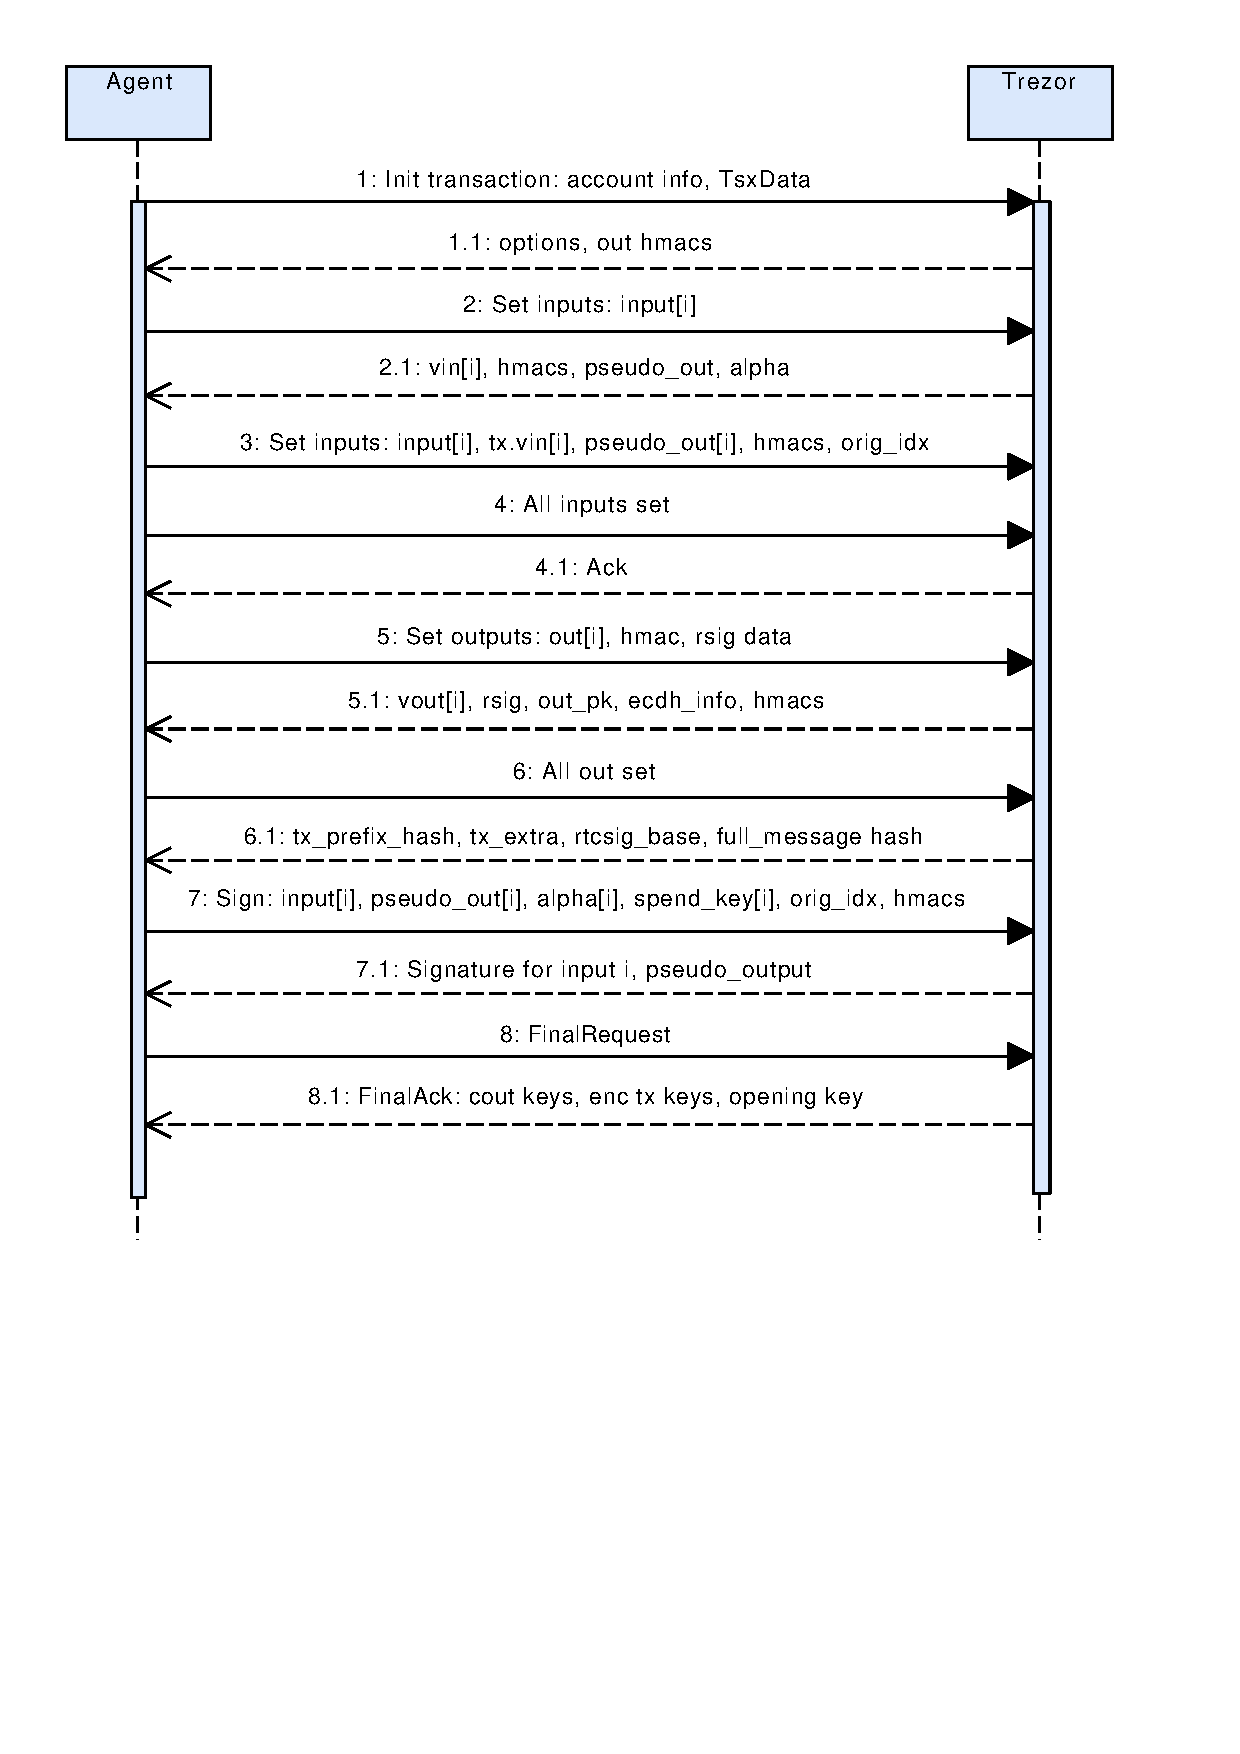
\includegraphics[width=0.8\textwidth,,trim={0 9cm 0 1cm},clip, angle=0]{img/subdivided.pdf}
	\caption{Subdivided protocol communication}
\end{figure}


The subdivided protocol description follows:

\begin{enumerate}
	\item Initialize the new protocol run as in the original one-step protocol. Send TsxData(version, payment\_id, unlock\_time, outputs, change\_dest, num\_inputs, mixin, fee, account\_id, minor\_indices).
	\begin{enumerate}
		\item Generate transaction master key $k_{mst} =  \textit{KDF}(TsxData \; || \; r \; || \; \text{rand\_nonce})$.
		
		\item Generate HMAC key $k_{hmac} = \textit{KDF}\left(\text{"hmac"} \; || \; k_{mst}\right)$
		
		\item Generate ENC key $k_{enc} = \textit{KDF}\left(\text{"enc"} \; || \; k_{mst}\right)$

		\item Generate HMAC for each output HMAC($\text{output}_i$) with the HMAC key: $\textit{KDF}(k_{hmac} \; || \; \text{"txdest"} \; || \; i)$ - the output pinning.
		
		\item Precompute sub-addresses. Construction data returned from watch-only wallet contain account ID (major sub-address index) and list of minor sub-addresses indices used in the transaction. Trezor precomputes sub-address spend keys.
		
		\item Return output HMACs.
	\end{enumerate} 

	\item $H \rightarrow T$: Send all transaction inputs $T_{in}$, one by one, as \verb|tx_source_entry|.\\
	$T_{in,i} = ((\text{idx}, P_j,C_j)_j, \text{amount}, \text{mask}, \pi, \text{pubs}, \dots)_i$
	\begin{enumerate}
		\item Trezor computes $x_{in}, \mathcal{D}_{in}, I_{in}$. The $x_{in}$ is stored in the Trezor transaction state. 
		If the number of inputs grows large the secret value 
		will have to be offloaded in an encrypted form.
		
		\item Compute transaction prefix field $tx.vin_i$, hash it incrementally to tx prefix hash.
		
		\item Compute HMAC on the data: HMAC($T_{in,i} \; || \; vin_i$), HMAC key: $\textit{KDF}(k_{hmac} \; || \; \text{"txin"} \; || \; i)$.
		
		\item Compute pseudo-out, i.e., Pedersen commitment on the UTXO amount. $ \text{pseudo\_out}_{in} = \alpha_{in} G + \text{amount}_{in} H$.
		
		\item Return $tx.vin_i$ part, HMAC($T_{in,i} \; || \; tx.vin_i$), $\text{pseudo\_out}_{in}$, HMAC($\text{pseudo\_out}_{in}$), Chacha20Poly1305($\alpha_{in}$)
	\end{enumerate} 

	\item $H \rightarrow T$: Set inputs permutation, inputs sorted by the key image. Permutation is represented as a simple integer array.
	
	\item $H \rightarrow T$: Send all transaction inputs $T_{in}$, one by one, as \verb|tx_source_entry|, with corresponding $tx.vin_i$ part and HMAC. Trezor verifies the HMAC and incrementally hashes $tx.vin_i$ to the \emph{transaction\_prefix\_hash}. Trezor also hashes $\text{pseudo\_out}_{in}$ to the RctSigBase.
	
	\item $H \rightarrow T$: Send all transaction outputs $T_{out}$, one by one, as \verb|tx_destination_entry|, together with corresponding HMAC generated in the init step. $T_{out,i} = ((A_d, B_d), \text{amount}, \dots)_i$. Change output $T_{chx}$ is the last transaction output if $T_{chx} \neq \perp$.
	\begin{enumerate}			
		\item Generate the key derivation $\mathcal{D}_{out}$, i.e., the \emph{amount key}.
		
		\item Derive a transaction output public key $P_{out} = H_s(\mathcal{D}_{out} || \text{varint}(\text{output\_index}))G + B_d$.
		
		\item Compute additional tx public keys $P_{out,j}$ if needed (sub-addresses).
		
        \item Compute the transaction prefix fields $tx.vout_i$ and $tx.extra_i$.
        
        \item Compute range proof on the output amount. \\
        - Generate scalar masks for each bit in the output amount $a_{i, j}, j \in [0, 63]$. \\
        - The range proof computes $C, rsig = \text{prove\_range}(a_{i, j}, amount_i)$, where $C$ is a Pedersen commitment on the output value: $C = \sum_{j}a_{i, j} G + amount_i H$. \\
        - Hash the range proof incrementally to the \emph{final\_message}.\\
        - Compute $\text{out\_pk}_i = \text{CtKey}(\text{dest}=tx.vout_i.output,\text{mask}=C)$.\\  
        - Compute $\text{ecdh\_info}_i$ masked with the \emph{amount key}. Plaintext data is $\text{amount}_i$ and mask $\sum_{j}a_{i, j}$. \\ \medskip
        - Hash the $\text{ecdh\_info}_i$ incrementally to the \emph{rct\_sig\_base} hash

        \item HMAC the output transaction data HMAC($T_{out,i} \; || \; tx.vout_i \; $) with HMAC key: $\textit{KDF}(k_{hmac} \; || \; \text{"txout"} \; || \; i)$.
                
        \item Store $tx.extra_i$, $\text{out\_pk}_i$ to the transaction state.
        
		\item Return the transaction prefix fields $tx.vout_i$ and $tx.extra_i$, $rsig_i$, $\text{out\_pk}_i$, $\text{ecdh\_info}_i$ and corresponding HMACs.
		
	\end{enumerate}
	  
	\item $H \rightarrow T$: All outputs set: The transaction prefix hash is computed and stored to the state. 
	
	\begin{enumerate}
		\item Check that sum of masks from the pseudo-outputs and output commitments are equal $\sum \alpha = \sum a_{i,j}$.
		
		\item Finalize incremental hashing of transaction prefix: hash $\text{out\_pk}_i$ from state. All \emph{final\_message\_hash} components are complete now. 
		
		\item Return transaction prefix hash, tx.extra, initial \emph{RctSig} structure
	\end{enumerate} 

	\item $H \rightarrow T$: Get full message hash. Trezor returns \emph{final\_message\_hash}.
	
	\item $H \rightarrow T$: RingCT Sign $T_{in}$. Send all transaction inputs $T_{in}$, one by one, with hmacs, pseudo output, alpha.
	\begin{enumerate}
		\item Check the HMAC
		
		\item Compute RingCT MG signature $S_i$ on the input and the \emph{final\_message}.
		
	\end{enumerate} 

	\item $H \rightarrow T$: Final message request. Responds with encrypted transaction keys. Keys are encrypted deterministically so they can be later decrypted and used if needed (e.g., spend proofs / tx proofs).
	
\end{enumerate}

% TODO: final message, encryption.

\paragraph{Alpha offloading}
The $\alpha_i$ mask values are required during signing (simple RCT variant with \#UTXO $\ge 1$). As the number of UTXO can be quite large the state memory does not have to be big enough to hold all masks. In that case we need to offload the alpha values to the host. 

The Chacha20Poly1305 is used with the key $\textit{KDF}\left(k_{enc} \; || \; \text{"txin-alpha"} \; || \; i\right)$. The $\alpha_i$ is then passed back to the Trezor in the signing phase. Alternative to offloading is deterministic mask generation described in section \ref{mask_reconstruction}.

A further research is needed to determine if encryption is needed or HMAC authentication is enough to preserve the security properties in the current attacker model, namely with no privacy guarantees on the host. As alpha values are not public by default the initial choice was to offload encrypted version, compared to the public values like range proofs, pseudo outputs and output public keys where HMAC is enough.

\paragraph{HMAC verification}
HMAC values are returned with the offloaded data to the host and verified when the offloaded values are loaded back to the Trezor. 
On HMAC failure transaction state is reset and user is notified the error happened.

%The message is generated by function \verb|get_pre_mlsag_hash|.
\subsection{Protocol selection}
The multi-step protocol is a generalization of the one-step version.
If the estimated size of the transaction is below a certain value (depends on $|T_{in}|, |T_{out}|, mixin$) the transaction is computed in one step to minimize the roundtrips. 

Multi-sig is not supported in the first implementation.

\subsection{State model}

State model of the transaction builder for incremental transaction signing. We assume many inputs (tens to hundreds, offloading to host) as balance can be scattered among many small UTXO while the output number is low (secrets kept in memory).

In the Figure \ref{fig:detailed_state} there is a hidden failed state. In case of an exception (e.g., HMAC error, invalid number of inputs, invalid message) the state is switched to the final Failed state. The failed state is not implemented explicitly as on the exception the transaction builder state is reset.

\begin{figure}[H]
	\centering
	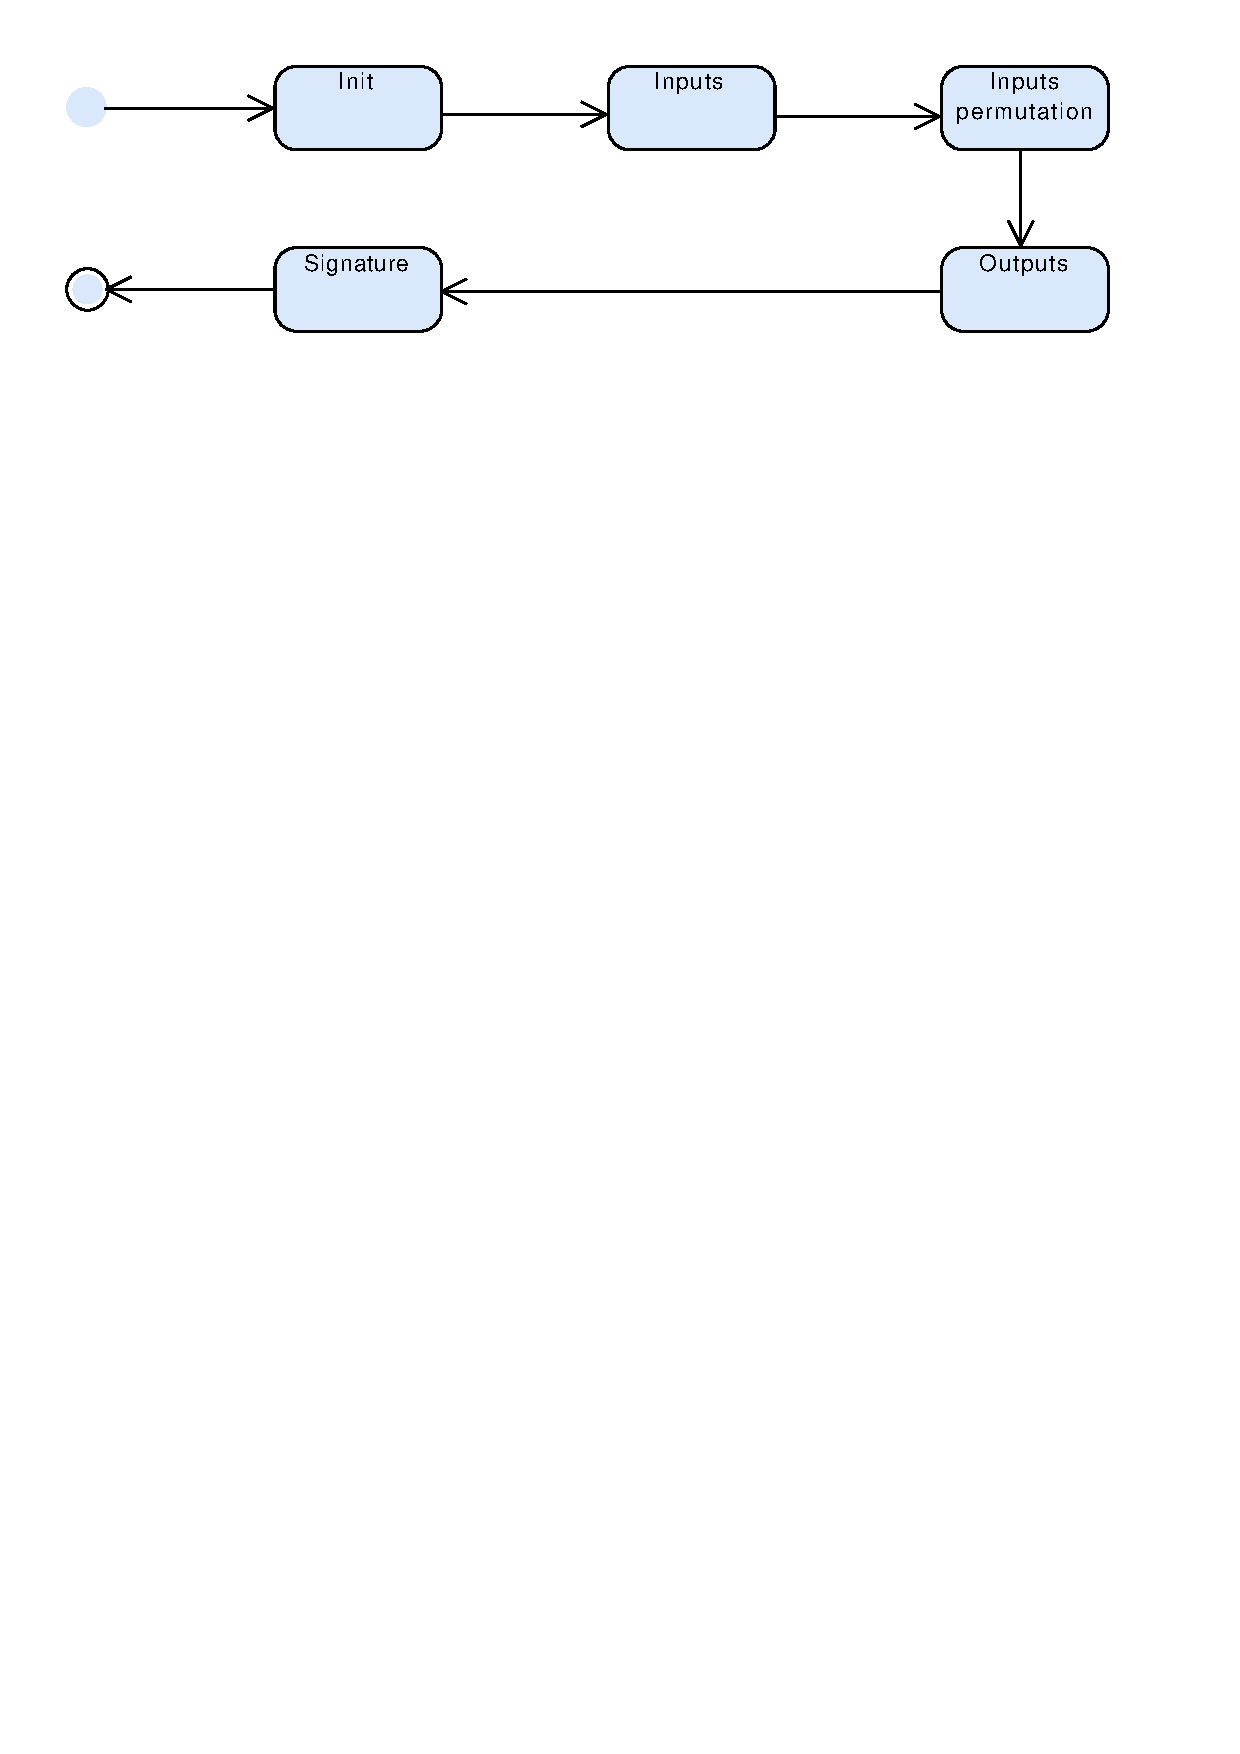
\includegraphics[width=0.6\textwidth,,trim={0 24cm 0 1cm},clip, angle=0]{img/tsx_state.pdf}
	\caption{Simplified transaction state for incremental signing}
\end{figure}

\begin{figure}[H]
	\centering
	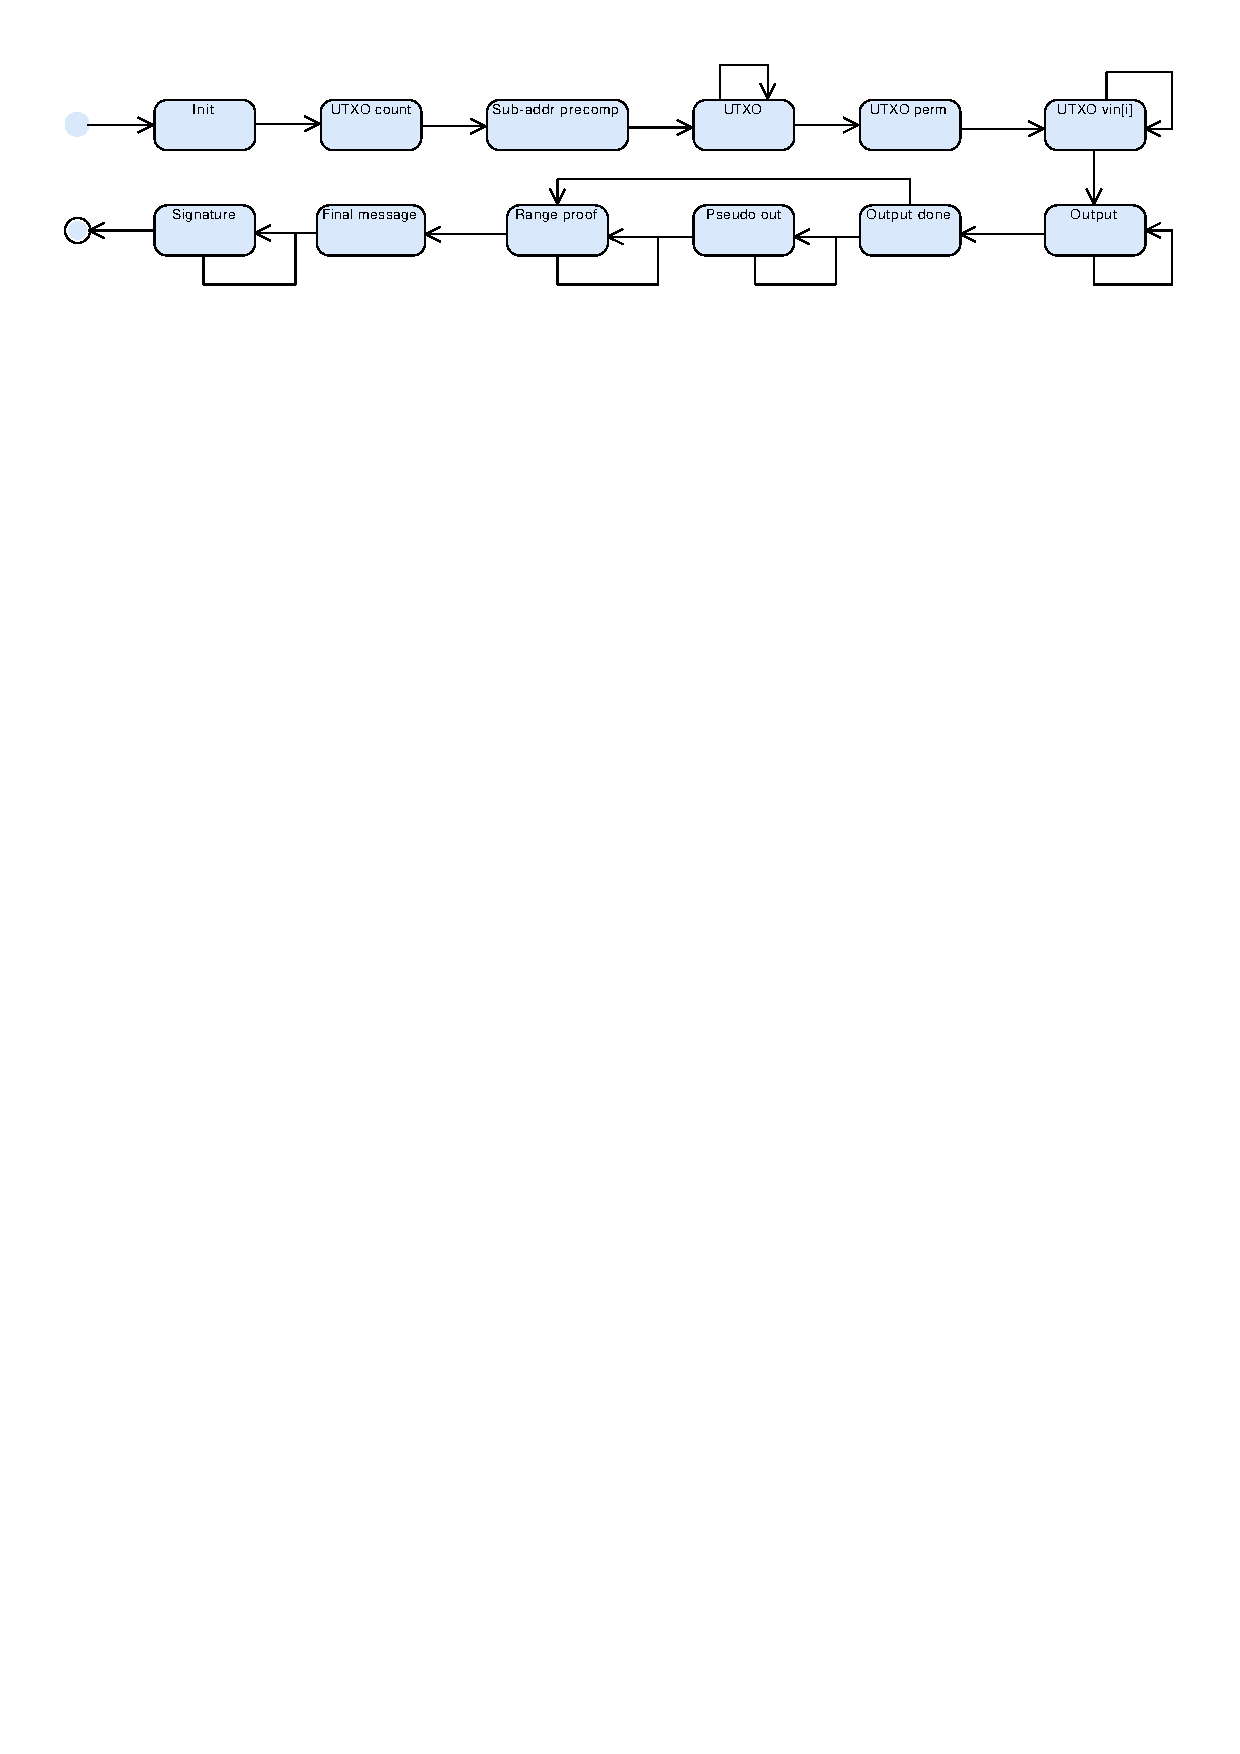
\includegraphics[width=1.\textwidth,trim={0 24cm 0 1cm},clip, angle=0]{img/tsx_state_detail.pdf}
	\caption{Detailed transaction state for incremental signing} \label{fig:detailed_state}
\end{figure}

\subsection{Signing data flow}
The illustrative data flow in the transaction signing is depicted in figure \ref{fig:data_flow}.

\begin{figure}[H]
	\centering
	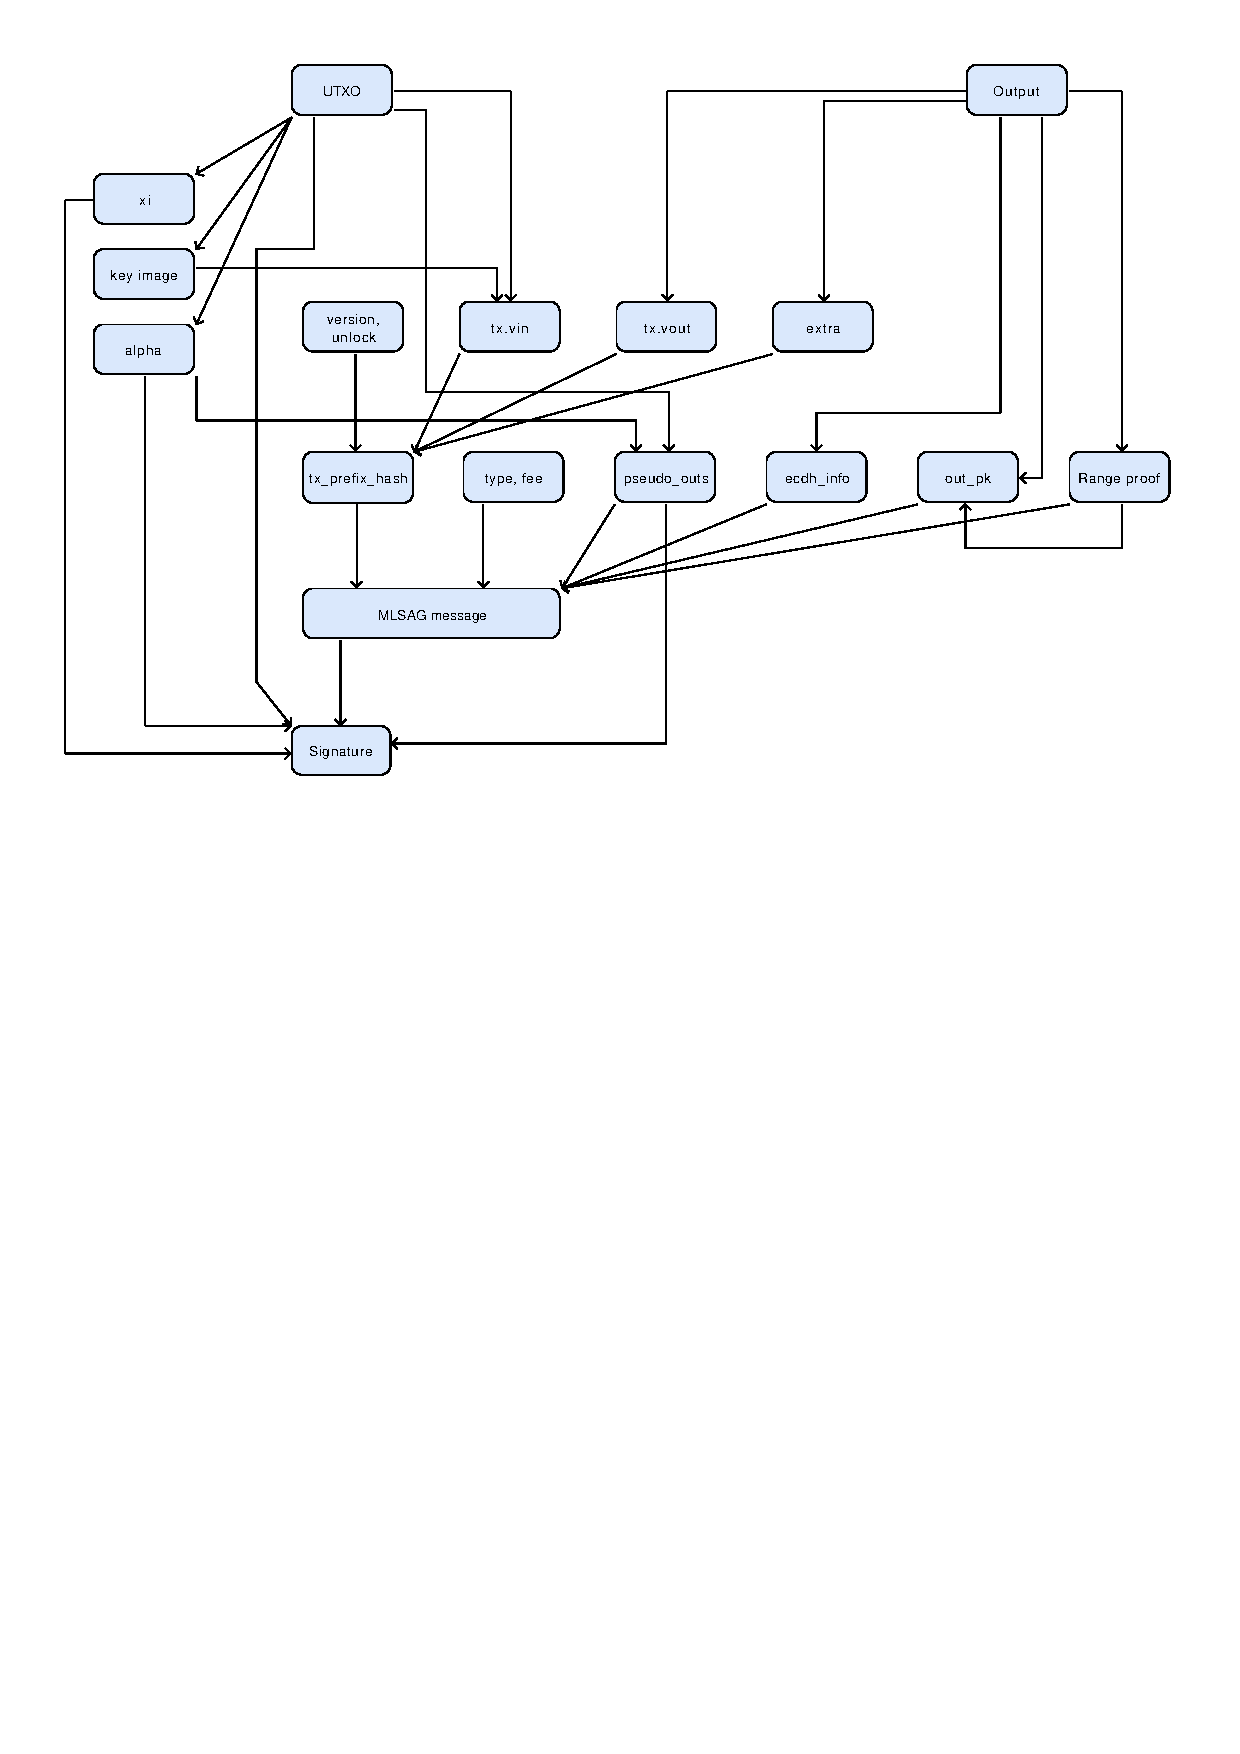
\includegraphics[width=1.\textwidth,trim={0 16cm 0 1cm},clip, angle=0]{img/data_flow.pdf}
	\caption{Data flow during signing} \label{fig:data_flow}
\end{figure}


\subsection{Borromean range proof computation in Trezor}
The range proof based on Borromean signatures consists of:
a) \emph{asig}.$s_0$ vector of 64 scalar values, 
b) \emph{asig}.$s_1$ vector of 64 scalar values,
c) \emph{asig}.$ee$ scalar value,
d) $C_i$ vector of 64 EC points, commitments.

\paragraph{Basic memory usage}
Assume the range proof is computed completely in the Trezor. Range proof itself consumes $(64 + 64 + 1) * 32 = 4128$~B for \emph{asig}, $64*32 = 2048$~B for $C_i$, commitments, $6176$~B in total.

Memory optimized variant of the range proof performs no additional precomputations, e.g., powers of $H$ are computed incrementally in constant memory. The range proof generates 64 random scalar masks $a_i$ used in commitment $C_i$ which is part of the range proof as shown in Figure \ref{eq:ci}. Moreover the Borromean signature generates another 64 random scalar mask values $\alpha_i$. The overall memory complexity estimate is thus $6176 + 64*32 + 64*32 = 10272$~B with neglecting constant overhead from counters and accumulators.  

\begin{figure}[H]
\begin{equation}
C_i = 
\begin{cases} 
a_iG & \text{bit(amount, i)} = 0 \\
a_iG + 2^iH & \text{bit(amount, i)} = 1 \\
\end{cases}
\end{equation}
\caption{$C_i$ Commitments} \label{eq:ci}
\end{figure}

\paragraph{Incremental version}
Trezor 2 has enough memory to compute range proof in one pass without modification. However, this is not necessarily true for devices with smaller RAM where some kind of incremental approach might be needed.

The naive incremental version computes range proof bit by bit, splitting it to 64 round-trips with minimal memory overhead per round-trip. The expected memory required for one round is roughly $10272 / 64 \approx 160$~B.

The Range proof generator algorithm cannot be trivially transformed to an incremental version as it requires 2 dependent passes over the 64 bits representing the amount. The symbolic range proof representation is illustrated by Algorithm \ref{alg:rangeproof}.

\begin{algorithm}[]
	\caption{Symbolic data flow in the Range proof} \label{alg:rangeproof}
	\begin{algorithmic}[1]
		\Function{RangeProof}{amount}
		\State $b \gets bits(amount)$
		\State $ee, sa, sC \gets 0, 0, O$
		\State $a, \alpha, C \gets 64 * 0, 64 * 0, 64 * O$
		\For{$i \in [0,63]$ }  \Comment{First pass}
			\State $a[i] \gets$ randomScalar()
			\State $\alpha[i] \gets$ randomScalar()
			\State $C[i], s1[i] \gets $ fncPass1($a[i], \alpha[i], b[i]$) \Comment{Depends only on the current round}
			\State $ee \gets \text{fncEe}(ee, C[i], s1[i])$ \Comment{$ee$ cross round dependency}
			\State $sa \gets sa + a[i]$ \Comment{Accumulators for commitments}
			\State $sC \gets \text{point\_add(sC, C[i])}$
		\EndFor
		
		\State $\;$
		\For{$i \in [0,63]$}  \Comment{Second pass}
			\State $s0[i], s1[i] \gets \text{fncPass2}(a[i], \alpha[i], b[i], C[i], s1[i], ee)$ \Comment{$ee$ dependency}
		\EndFor \\
		
		\Return{$sa, sC, C, s0, s1, ee$}
		\EndFunction	
	\end{algorithmic}
\end{algorithm}

Note the first pass generates all random values used in the range proof. Round results $C[i], s1[i]$ depend only on the current round values. The $ee$ which is needed for pass two accumulates information from each round. There are two more accumulators needed for commitments, $sa, sC$.
The first pass is trivially parallelizable.
Also note the second pass rounds use only information for the particular round, besides accumulator $ee$.
The second pass makes use of generated random scalar masks. In the following paragraphs there are two possible incremental transformations presented.

\paragraph{Deterministically generated masks} \label{par:det_masks}
As scalar masks $a, \alpha$ are used in the second pass rounds the incremental version has to have an access to those values. Masks can be either stored in the memory, but this requires $128*32 = 4096$~B storage.
To overcome this issue we can use deterministic mask generation as described in \ref{par:det_masks} as shown in Figure \ref{eq:masks}. In this way the second pass can regenerate the same mask values $a, \alpha$ as were used in the first pass.

\begin{figure}[H]

	\begin{equation}
	\begin{split}
	k_{\textit{rsig0,idx}} &= \textit{KDF}\left(k_{msk} \; || \; \text{"rsig-rnd-ai"} \; || \; idx \right)\\
	k_{\textit{rsig1,idx}} &= \textit{KDF}\left(k_{msk} \; || \; \text{"rsig-rnd-alphai"} \; || \; idx \right)\\
	a[i] &= \textit{KDF}(k_{\textit{rsig0,idx}} \; || \; i \; ) \; \text{mod} \; l  \\
	\alpha[i] &= \textit{KDF}(k_{\textit{rsig1,idx}} \; || \; i \; ) \; \text{mod} \; l
	\end{split}
	\end{equation}

	\caption{$a[i], \alpha[i]$ Generation. $idx$ is the output index in the transaction, $l$ is Ed25519 generator order.} \label{eq:masks}
\end{figure}

The first pass it trivially converted to incremental version, returning $s1[i], C[i]$ with HMAC for each finished round. 
After the first pass is finished the $sA, sC, ee$ is returned. The second pass round takes $s0[i], C[i]$ as an input, checks the HMAC and computes corresponding $s0[i], s1[i]$. 

%\paragraph{63-of-64.} In this idea the 63 out of 64 mask are generated deterministically 
% TODO: 63-of-64 bits, conceal final mask value, ee problem - hashing, handover hashing state.

\paragraph{Memory Offloading}
Another variant makes use of offloading an encrypted version of masks to the host.
Masks are generated randomly in the Trezor as in the original algorithm.
The first pass round returns $s1[i], C[i], \text{Chacha20Poly1305}(a[i], \alpha[i])$.
The second pass takes result of the first pass and produces $s0[i], s1[i]$.

\paragraph{Slicing} 
The naive incremental algorithm performs $2 * 64$ round trips. The trade-off between round trips and memory can be adjusted by batching some number of bit rounds together, depending on the amount of free memory. 

\paragraph{Incremental hashing}
Due to the \emph{final\_message} hash structure it is not possible to incrementally hash range proof during the generation time per bits. The second pass can hash all $s0$ but then we need to hash all $s1$, $ee$ and all $C$. The additional protocol round trips are needed to finish range proof hashing to the \emph{final\_message}. The range proof section is independent on other \emph{final\_message} sections thus its doable just after the range proof generation is finished. To avoid tampering of the computed values the $s1, ee, C$ have to be HMACed. The same batching applies as described in the previous paragraph. 

\subsection{Protocol extension - host computed range signature}

Mainly due to the reasons given in the section \ref{sec:bp} it is needed to offload the range signature to the host, especially if batched Bulletproofs are used. Single Borromean and Bulletproof can be generated on the Trezor which simplifies the protocol. If computation on the Trezor cannot be done the offloading has to be employed. 
Several different offloading mechanisms have been described. We aim for the general protocol design so it can carry out different possible offloading. 

The main idea: 
\begin{itemize}
	\item After all inputs are set, the total mask sum is computed, the Trezor can compute commitment masks for the outputs and further output and range sig parameters.
	A new roundtrip is thus added where Trezor instructs host about the range sig parameters. This requires a new message roundtrip. 
	
	\item If the range sig offloading strategy allows it, the host can compute rangesig directly and send it with the \emph{MoneroTransactionSetOutputRequest} message. 
	
	\item If the offloading is more complicated, host sends \emph{MoneroTransactionSetOutputRequest} message as normally. The response contains \emph{MoneroRsigData} message. It can contain partially computed rsig. If necessary there may be several \emph{MoneroRsigData} roundtrips until whole rsig is computed. After the computation the Trezor has rsig hash so it can finish computation of the pre MLSAG hash required for the signature.
\end{itemize} 

For the purpose of offloading we define a new general message \emph{MoneroRsigData}:

\begin{lstlisting}
message MoneroRsigData {
  optional uint32 version = 1;
  optional uint32 step = 2;
  optional uint64 operation = 3;
  optional bytes seed = 4;   // determ. mask seed
  optional bytes mask = 5;   // mask vector
  optional bytes amount = 6; // amount vector
  optional bytes rsig = 7;   // range sig, full or partial
  repeated MoneroTransactionDestinationEntry outputs = 8;
}

\end{lstlisting}

\begin{figure}[H]
	\centering
	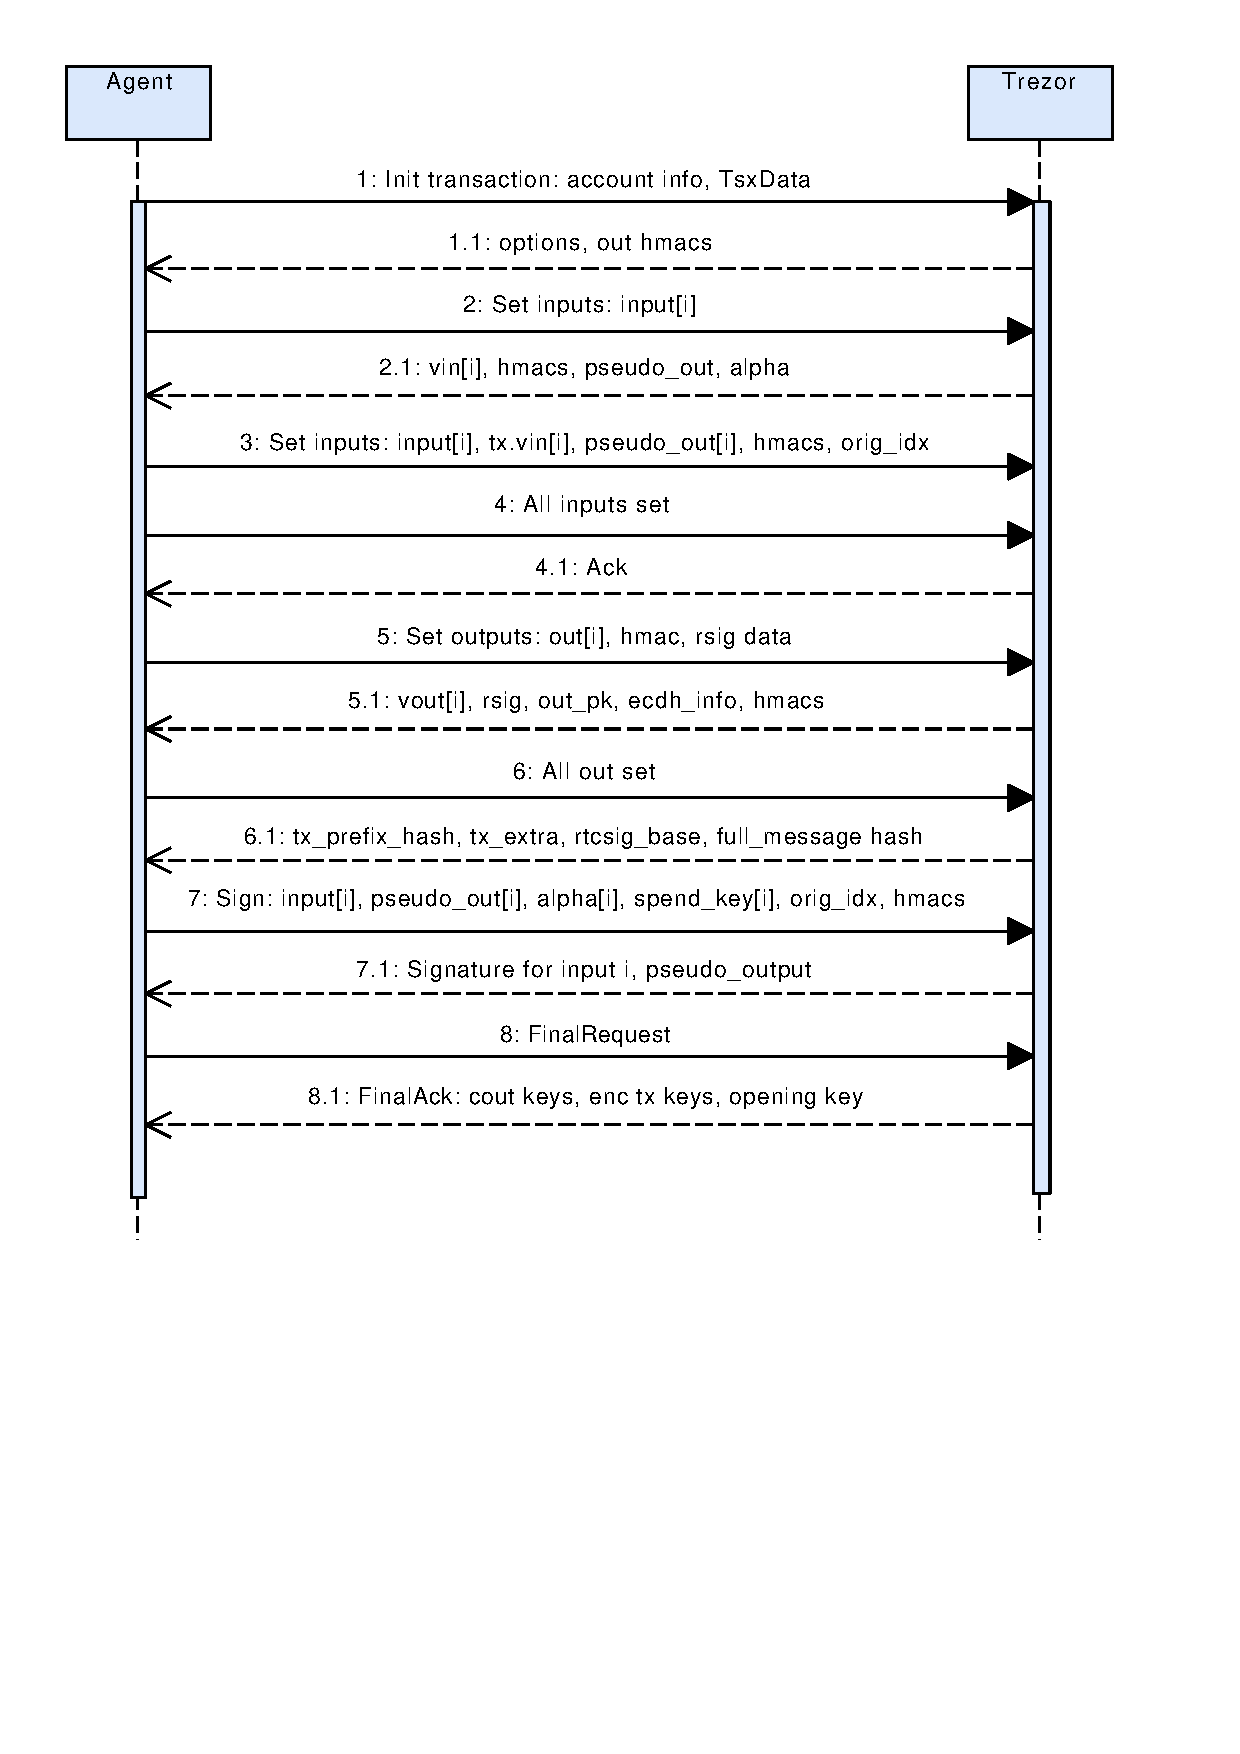
\includegraphics[width=0.8\textwidth,,trim={0 3cm 0 1cm},clip, angle=0]{img/subdivided_rsig.pdf}
	\caption{Extended protocol with range sig offloading}
\end{figure}

\begin{figure}[H]
	\centering
	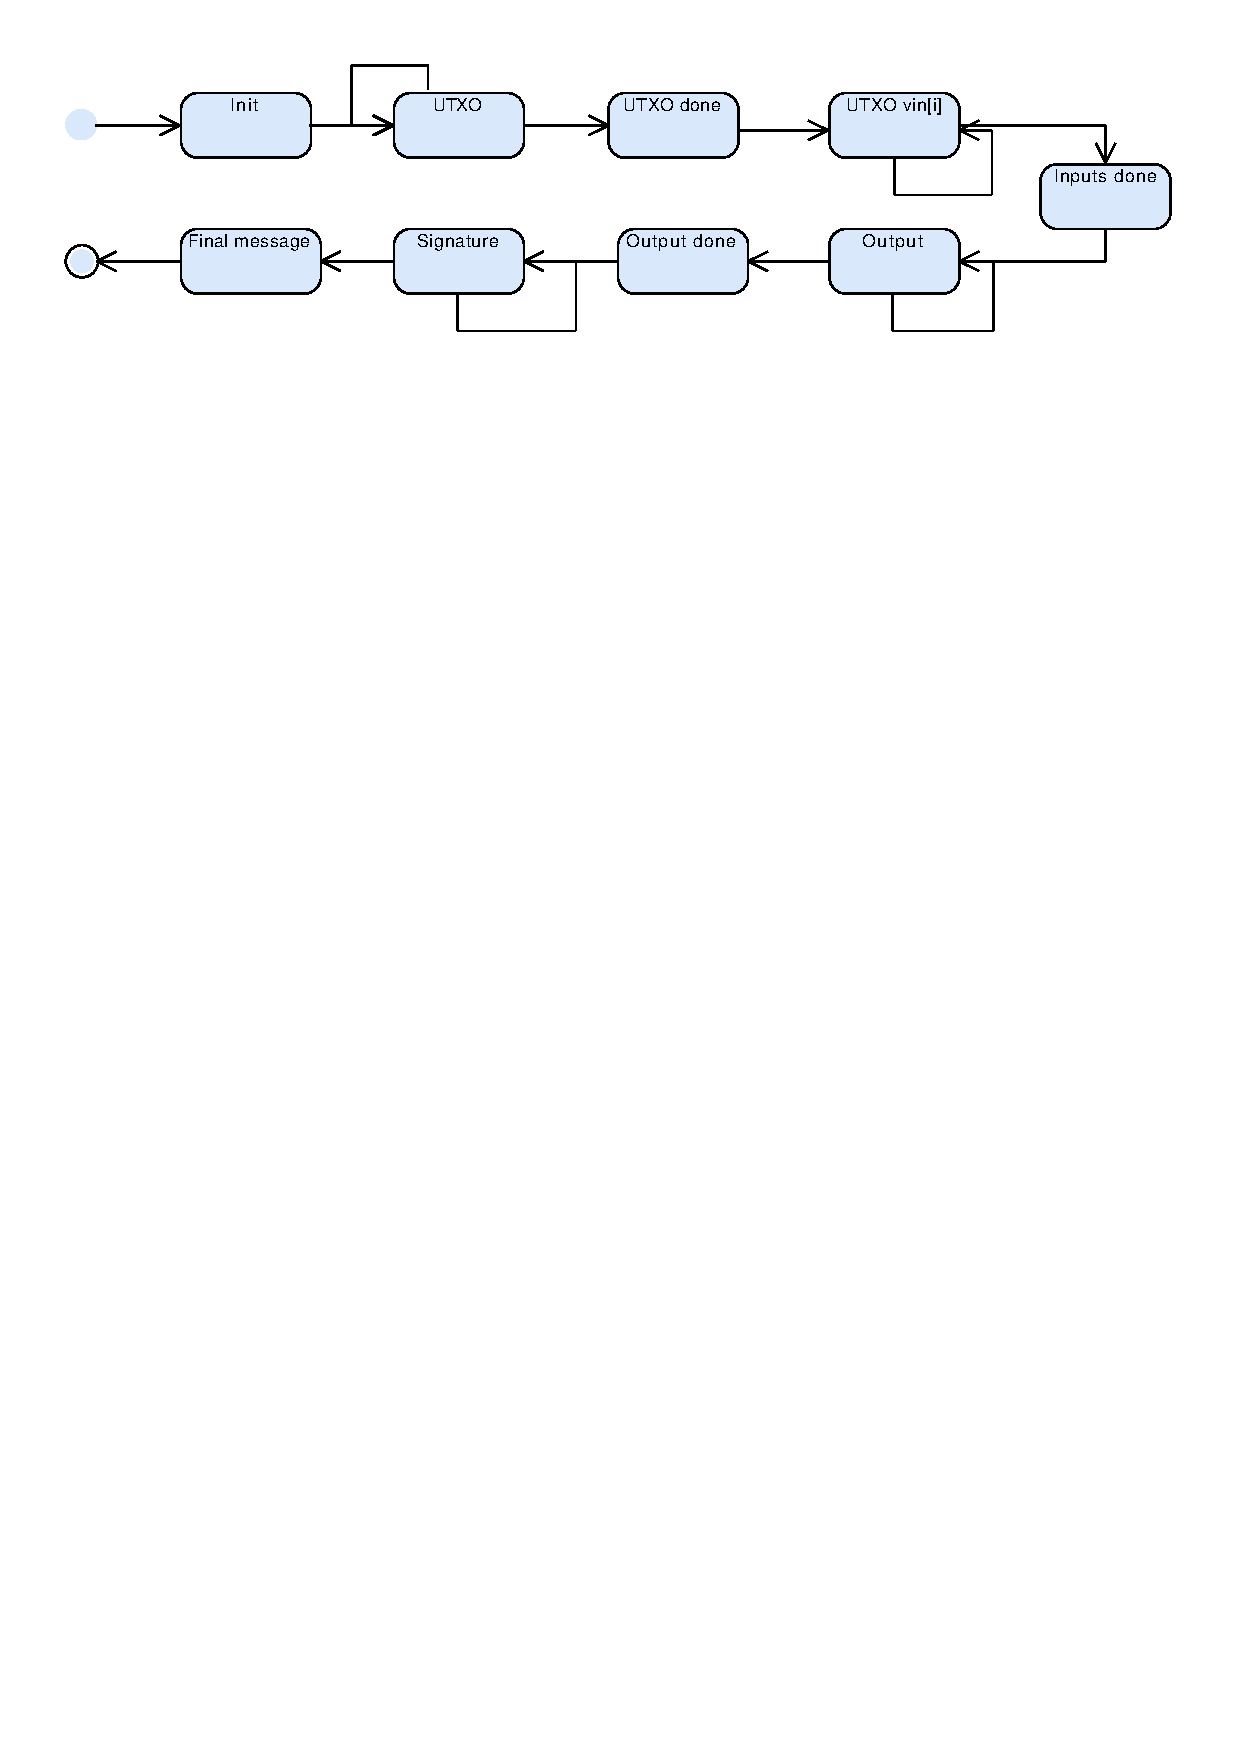
\includegraphics[width=1.\textwidth,trim={0 22cm 0 1cm},clip, angle=0]{img/tsx_state_detail_rsig.pdf}
	\caption{State machine for incremental signing with range sig offloading} \label{fig:detailed_state}
\end{figure}


\section{Implementation}

The implementation process is incremental, start with MVP, minimal viable product. Later extend with more features. MVP has two basic features: 1) receive transactions, view balance, 2) send transaction. 

Receiving transactions does not require Trezor interaction as the view key is exported to the software wallet. Sending a transaction required Trezor interaction.

\;
\noindent Basic implementation steps:
\begin{enumerate}
	\item Trezor basic Monero-related ed25519 crypto
	\item Transaction specific crypto-material derivation
	\item Monero binary serialization
	\item Monero specific messages for Trezor-Host interface
	\item RingCT and basic transaction primitives
	\item Monero transaction assembly
	\item Extend simplewallet to support Trezor
	\item Monero wallet for Trezor.io 
\end{enumerate}

\subsection{Watch-only full wallet}
The integration idea is to do minimal modifications to the official Monero codebase so the integration maintainability and merge probability are increased. We aim to add minimal feature set required for our use case to the Monero codebase. 

\paragraph{Watch-only wallet and Trezor client} 
The wallet having only view key available is called watch-only wallet. It performs the blockchain scanning for the user, stores all UTXO, communicates with the full-node, assembles the transaction inputs for a new transfer but the signatures have to be done in the full-fledged wallet with the spend key. 

Monero wallet supports a cold-wallet scenario where the transaction is prepared in the watch-only wallet, so called \emph{unsigned transaction}, and the signature is performed in the cold-wallet. Trezor integration make use of this functionality to do the signature. In order to decouple Trezor specific code from the official Monero codebase there is another software module added, Trezor software client facilitating the communication and the protocol itself. The client can be later integrated to the Monero codebase or run standalone and communicate over a socket.

\begin{figure}[H]
	\centering
	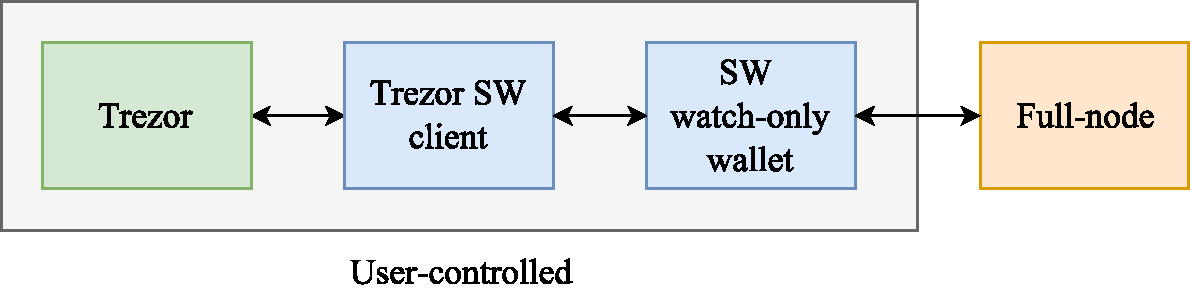
\includegraphics[width=0.6\textwidth, angle=0]{img/trezor-int.pdf}
	\caption{Environment with the Trezor client}
\end{figure}

\paragraph{Unsigned transaction.}
The watch-only wallet exports \verb|struct unsigned_tx_set| encrypted with the view key which is imported in the fully-fledged wallet, decrypted, and signed. Here follows the overview of the \verb|unsigned_tx_set| structure and related types.

\begin{lstlisting}[language=c++]
// UTXO vector
typedef std::vector<transfer_details> transfer_container;

// Data for signing one transaction
struct tx_construction_data {
  std::vector<cryptonote::tx_source_entry> sources;
  cryptonote::tx_destination_entry change_dts;
  
  // split, includes change
  std::vector<cryptonote::tx_destination_entry> splitted_dsts; 
  std::vector<size_t> selected_transfers;
  std::vector<uint8_t> extra;
  uint64_t unlock_time;
  bool use_rct;
  
  // original setup, does not include change
  std::vector<cryptonote::tx_destination_entry> dests; 
  
  // subaddress account of your wallet to be used in this transfer
  uint32_t subaddr_account;  
  
  // set of address indices used as inputs in this transfer
  std::set<uint32_t> subaddr_indices;  
}

// Unsigned transaction set
struct unsigned_tx_set {
  std::vector<tx_construction_data> txes;
  wallet2::transfer_container transfers;
};
\end{lstlisting}

\paragraph{SW wallet integration.} The software wallet can be either linked to the wrapping project or RPC calls can be used. The linking enables to use \verb|wallet2_api.h|\footnote{\url{https://github.com/monero-project/monero/blob/master/src/wallet/api/wallet2_api.h}} and \verb|wallet_manager.h|\footnote{\url{https://github.com/monero-project/monero/blob/master/src/wallet/api/wallet_manager.h}} which is simpler to use rather than \verb|wallet_rpc_server.h|\footnote{\url{https://github.com/monero-project/monero/blob/master/src/wallet/wallet_rpc_server.h}} which requires serialization but provides greater flexibility.

In the following sections the signature integration schemes are proposed.

\subsection{Variant A - interaction with the monero-wallet-cli}
In this variant a user interacts with the traditional Monero wallet software running as watch-only wallet, either CLI or the GUI extension. Trezor client is a module in the software wallet and wallet has to be configured to use the Trezor. 
The benefit is users use existing interfaces with minimal changes and learning new UX.
The downside is the monero wallet has to be able to call the signing method on the Trezor client to sign the transaction.

\begin{itemize}
	\item Wallet communicates with the node in several round-trips. Outputs frame groups the whole communication.
	\item Step 1.3 the sign call passes \verb|unsigned_tx_set| structure to the Trezor client. 
	\item Protocol frame encapsulates the whole signature protocol as described above. Trezor client implements the signature protocol. There can be several message round-trips in the protocol.
	\item Trezor client returns all signed transactions to the software wallet which submits them to the full node.
	\item The client can a) run standalone on a socket, b) be invoked as an external program, c) be integrated as a shared lib / plugin to the Monero codebase. If the client runs as an external application users need to install another piece of software which can be quite a hassle.
\end{itemize}
 
\begin{figure}[H]
	\centering
	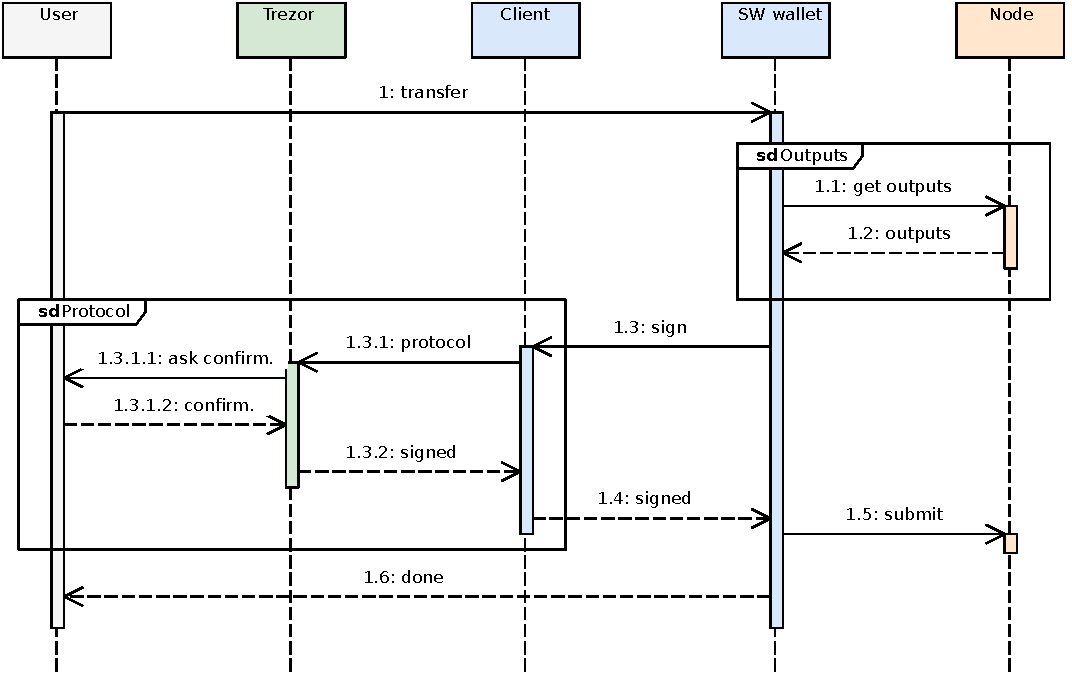
\includegraphics[width=0.9\textwidth, angle=0]{img/variantA.pdf}
	\caption{Interaction sequence variant A}
\end{figure}

Changes required in this scenario are mainly related to the step 1.3. SW wallet has to be able to call the client (RPC/.so func call). Wallet has to be configured to run with the Trezor client.

\subsection{Variant B - interaction with the client}
This variant assumes the main entry point is the Trezor client which calls software watch-only Monero wallet, either via RPC or via .so func call (wallet2 linked to the client). The Trezor client forms a wrapper for the official Monero wallet. The wrapper can initialize the software wallet in watch-only mode with the view-key exported so the configuration hassle is reduced compared to the previous variant. This variant also enables to quickly proof the concept of the signature protocol with minimal code changes to the Monero code base. 

Linking the official wallet code rather than using RPC methods is faster in terms of implementation for the initial PoC as no serialization and new RPC methods are needed to be added to the Monero code. Once the linking scenario is implemented the RPC extension using newly implemented functions is added which provides greater flexibility and decoupling.

The linking also enables to use original CLI wallet interface with overriding only spend-key related commands by extending the \verb|simple_wallet| class. Other commands can be proxied to the software wallet. This preserves the UX for the user while enabling flexibility using the Trezor for signing. Linking approach is also used by other Monero wallets, e.g. \emph{monerujo.io}.\footnote{\url{https://github.com/m2049r/xmrwallet}}

\begin{figure}[H]
	\centering
	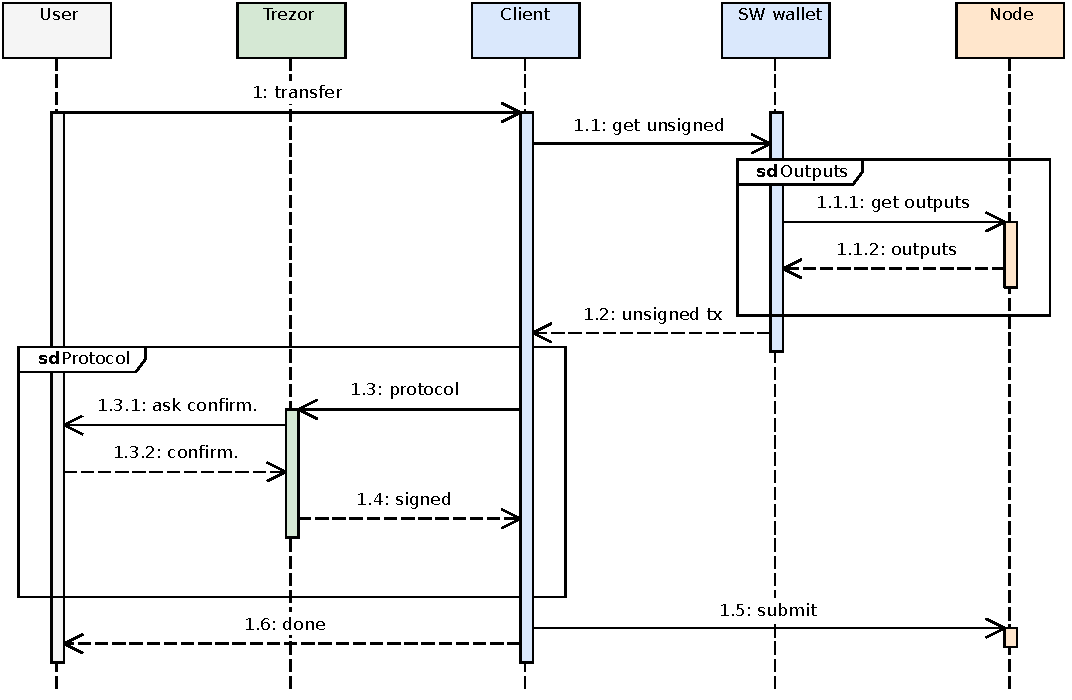
\includegraphics[width=0.9\textwidth, angle=0]{img/variantB.pdf}
	\caption{Interaction sequence variant B}
\end{figure}

This variant does not require changing the software wallet.
Only the small portion of the \verb|simple_wallet| is reimplemented in the client, namely \verb|simple_wallet::transfer_main()| function.

Trezor client uses \verb|wallet2::create_transactions_2| to create pending transaction which can be later signed by the signature protocol.

\begin{lstlisting}[language=c++]
std::vector<wallet2::pending_tx> wallet2::create_transactions_2(
  std::vector<cryptonote::tx_destination_entry> dsts, 
  const size_t fake_outs_count, 
  const uint64_t unlock_time, 
  uint32_t priority, 
  const std::vector<uint8_t>& extra, 
  uint32_t subaddr_account, 
  std::set<uint32_t> subaddr_indices, 
  bool trusted_daemon)
\end{lstlisting}


\subsection{Memory considerations}
Python uses arbitrary precision integers with a memory overhead.
The following command shows the amount of memory required for certain data types and sizes:
\begin{lstlisting}[language=python]
>>> sys.getsizeof(0)
24
>>> sys.getsizeof(2**32-1)  # 4B num
32
>>> sys.getsizeof(2**64-1)  # 8B num
36
>>> sys.getsizeof(2**256-1)  # 32B num
60
>>> sys.getsizeof(b'\x00'*32)  # 32B hex
65
>>> sys.getsizeof(b'\x00'*64)  # 64B hex
97
\end{lstlisting}

Monero works in EC with 32 B numbers. To store a 32 B number it takes 60 B in integer representation and 65 B in the byte string encoded representation (some ed25519 libraries and mininero use this representation). For scalars it is apparently more effective to store integers naturally, saving both memory and CPU cycles with recoding.

EC point arithmetics can use classic point coordinates $(x, y)$ or extended Edwards point coordinates $(x,y,z,t)$. It takes 64 and 80 B to store tuple of 2 and 4 elements respectively. It thus take 184 B and 320 B to store an EC point in the natural form compared to the 65 B byte representation.


\section{Trezor.io}

The more complex integration scenario - trezor.io software wallet.
\begin{enumerate}
	\item Chrome plugin - communication channel to the Trezor device. 
	JS interface to the Trezor. Minimal changes, add new Monero-related messages.
	
	\item Trezor.io Monero RPC node. Full-node local vs. remote node (trusted). A user can run his local node. The node is set in the trezor.io menu. By default, there can be an implicit node owned by the SatoshiLabs or Monero open nodes. So far it seems we don't need blockchain explorer (such as Insight for BTC). The RPC interface of the monero full-node seems enough for the initial version.
	
	\item Basic Monero JS wallet for Trezor.io. Minimalistic for a start. Simple receive + send (spending proofs, etc. can be added later or by the community). 
	
	\item Trezor.io wallet stores transfers, does transaction scanning, wallet refresh, communicates with the full-node (refresh, fake get outs). Range proof could be implemented in the Trezor directly for this case. 
	
	\item Implement Monero crypto in JS. Basic Monero-specific ed25519 operations, SHA-3 based $H_s(), H_p()$.
	
\end{enumerate}


%\section{Current progress}
%The current state of the work:
%
%\begin{itemize}
%	\item Finishing the feasibility study and the analysis of the Monero and Trezor.
%	\item 
%\end{itemize}


%\improvement[inline]{Add more}

\appendix
\section{Example of Monero transactions}

\lstdefinestyle{jsonStyle}{
	numbers=left,
	stepnumber=1,
	tabsize=4,
	showspaces=false,
	showstringspaces=false
}

\lstset{
	string=[s]{"}{"},
	stringstyle=\color{blue},
	comment=[l]{:},
	commentstyle=\color{black},
	style=jsonStyle
}

Few examples with full json transcript:
\begin{itemize}
	\item \footnotesize\url{https://xmrchain.net/tx/599533a7e42e82aa23c8da1d730fec047915ee5614556883cdce90739f1a94d3/1}
	
	\item \footnotesize\url{https://xmrchain.net/tx/84d09b596cf847eefd5a17ff9eb493e6f33f0a5e601b775e33831cdd6cadf53d/1}
	
	\item \footnotesize\url{https://xmrchain.net/tx/5620d6c7e425ad53d3228f4b70adac0d798915a6d049079a3795dbda5b2b0cce/1}
	
	\item \footnotesize\url{https://xmrchain.net/tx/ae52a85bebaae2a488071aaf0dfbaf143148fd943a8d5f659e2c8ad61e69a318/1}
\end{itemize}

\section{Structure definitions} \label{sec:structs}


\lstset{
	%string=[s]{"}{"},
	%stringstyle=\color{blue},
	comment=[l]{:},
	commentstyle=\color{gray},
	style=cstyle
}

\begin{lstlisting}[language=c++]

// 
// File: src/crypto/crypto.h
// 

struct ec_point {
  char data[32];
};

struct ec_scalar {
  char data[32];
};

struct public_key: ec_point {
};

//
// File: src/cryptonote_basic/cryptonote_basic.h
// 

struct account_public_address {
  crypto::public_key m_spend_public_key;
  crypto::public_key m_view_public_key;
}

struct txout_to_script {
  std::vector<crypto::public_key> keys;
  std::vector<uint8_t> script;
};

struct txout_to_scripthash {
  crypto::hash hash;
};

struct txout_to_key {
  crypto::public_key key;
};


struct txin_gen {
  size_t height;
};

struct txin_to_script {
  crypto::hash prev;
  size_t prevout;
  std::vector<uint8_t> sigset;
};

struct txin_to_scripthash {
  crypto::hash prev;
  size_t prevout;
  txout_to_script script;
  std::vector<uint8_t> sigset;
};

struct txin_to_key {
  uint64_t amount;
  std::vector<uint64_t> key_offsets;
  crypto::key_image k_image;  
};

typedef boost::variant<txin_gen, txin_to_script, txin_to_scripthash, 
  txin_to_key> txin_v;

typedef boost::variant<txout_to_script, txout_to_scripthash, 
  txout_to_key> txout_target_v;


struct tx_out {
  uint64_t amount;
  txout_target_v target;
};

class transaction_prefix {
  size_t   version;
  uint64_t unlock_time; 
  std::vector<txin_v> vin;
  std::vector<tx_out> vout;
  std::vector<uint8_t> extra;
};

//
// File: src/ringct/rctTypes.h
//

struct key {
  unsigned char bytes[32];
};

typedef std::vector<key> keyV; //vector of keys
typedef std::vector<keyV> keyM; //matrix of keys (indexed by column first)

struct ctkey {
  key dest;
  key mask;
};

typedef std::vector<ctkey> ctkeyV;
typedef std::vector<ctkeyV> ctkeyM;

// Used for multisig data
struct multisig_kLRki {
  key k;
  key L;
  key R;
  key ki;
};

struct ecdhTuple {
  key mask;
  key amount;
}

typedef key key64[64];
struct boroSig {
  key64 s0;
  key64 s1;
  key ee;
};

struct mgSig {
  keyM ss;
  key cc;
  keyV II;
};

struct rangeSig {
  boroSig asig;
  key64 Ci;
};

struct Bulletproof
{
  rct::keyV V;
  rct::key A, S, T1, T2;
  rct::key taux, mu;
  rct::keyV L, R;
  rct::key a, b, t;
}

struct rctSigBase {
  uint8_t type;
  key message;
  ctkeyM mixRing; //the set of all pubkeys / copy
  keyV pseudoOuts;
  std::vector<ecdhTuple> ecdhInfo;
  ctkeyV outPk;
  xmr_amount txnFee;
}

struct rctSigPrunable {
  std::vector<rangeSig> rangeSigs;
  std::vector<Bulletproof> bulletproofs;
  std::vector<mgSig> MGs; // simple rct has N, full has 1
  keyV pseudoOuts; //C - for simple rct
}

struct rctSig: public rctSigBase {
  rctSigPrunable p;
};

//
// File: src/cryptonote_core/cryptonote_tx_utils.h
//

struct tx_source_entry
{
  typedef std::pair<uint64_t, rct::ctkey> output_entry;

  std::vector<output_entry> outputs;  //index + key + optional ringct commitment
  size_t real_output;                 //index in outputs vector of real output_entry
  crypto::public_key real_out_tx_key; //incoming real tx public key
  std::vector<crypto::public_key> real_out_additional_tx_keys; //incoming real tx additional public keys
  size_t real_output_in_tx_index;     //index in transaction outputs vector
  uint64_t amount;                    //money
  bool rct;                           //true if the output is rct
  rct::key mask;                      //ringct amount mask
  rct::multisig_kLRki multisig_kLRki; //multisig info
}

struct tx_destination_entry
{
  uint64_t amount;                    //money
  account_public_address addr;        //destination address
  bool is_subaddress;
}

// 
// File: src/wallet/wallet2.h
//

struct multisig_info {
  struct LR {
    rct::key m_L;
    rct::key m_R;
  };

  crypto::public_key m_signer;
  std::vector<LR> m_LR;
  
  // one per key the participant has
  std::vector<crypto::key_image> m_partial_key_images; 
};

struct transfer_details {
  uint64_t m_block_height;
  cryptonote::transaction_prefix m_tx;
  crypto::hash m_txid;
  size_t m_internal_output_index;
  uint64_t m_global_output_index;
  bool m_spent;
  uint64_t m_spent_height;
  crypto::key_image m_key_image; 
  rct::key m_mask;
  uint64_t m_amount;
  bool m_rct;
  bool m_key_image_known;
  size_t m_pk_index;
  cryptonote::subaddress_index m_subaddr_index;
  bool m_key_image_partial;
  std::vector<rct::key> m_multisig_k;
  std::vector<multisig_info> m_multisig_info; // one per other participant
}

struct tx_construction_data{
  std::vector<cryptonote::tx_source_entry> sources;
  cryptonote::tx_destination_entry change_dts;
  
  // split, includes change
  std::vector<cryptonote::tx_destination_entry> splitted_dsts; 
  std::vector<size_t> selected_transfers;
  std::vector<uint8_t> extra;
  uint64_t unlock_time;
  bool use_rct;
  
  // original setup, does not include change
  std::vector<cryptonote::tx_destination_entry> dests; 
  
  // subaddress account of your wallet to be used in this transfer
  uint32_t subaddr_account;   
  
  // set of address indices used as inputs in this transfer
  std::set<uint32_t> subaddr_indices;  
}

typedef std::vector<transfer_details> transfer_container;
typedef std::unordered_multimap<crypto::hash, payment_details> payment_container;

struct multisig_sig {
  rct::rctSig sigs;
  crypto::public_key ignore;
  std::unordered_set<rct::key> used_L;
  std::unordered_set<crypto::public_key> signing_keys;
  rct::multisig_out msout;
};

struct pending_tx
{
  cryptonote::transaction tx;
  uint64_t dust, fee;
  bool dust_added_to_fee;
  cryptonote::tx_destination_entry change_dts;
  std::vector<size_t> selected_transfers;
  std::string key_images;
  crypto::secret_key tx_key;
  std::vector<crypto::secret_key> additional_tx_keys;
  std::vector<cryptonote::tx_destination_entry> dests;
  std::vector<multisig_sig> multisig_sigs;

  tx_construction_data construction_data;
}

struct unsigned_tx_set {
  std::vector<tx_construction_data> txes;
  wallet2::transfer_container transfers;
};

struct signed_tx_set {
  std::vector<pending_tx> ptx;
  std::vector<crypto::key_image> key_images;
};

struct multisig_tx_set {
  std::vector<pending_tx> m_ptx;
  std::unordered_set<crypto::public_key> m_signers;
};

\end{lstlisting}

% References
\bibliography{monero}{}
\bibliographystyle{plain}
	
\end{document}

